\coverchapter{Strategies for TileScope}\label{ch:strats}
This chapter introduces three new strategies for TileScope, column reverse, column permutation and sliding. The first two, although perfectly valid strategies on their own, are used to extend sliding to any columns. The sliding strategy, as previously mentioned, allowed for the first discovery of a specification for $\Av{1432}$ by TileScope. 

Using a specification for $\Av{1234}$ discovered by TileScope and applying the same strategies at every step starting with $\Av{1432}$, we had a matching tree except for one tiling that we failed to expand in the same manner as the one for $\Av{1234}$. By looking at the tree we had created from the $\Av{1432}$ root, we could see what tiling was needed instead of the one we failed to expand in order to complete the specification in the same way. This pair of tilings, shown in \FigureRef{fig:slidepair}, whose inconspicuous equivalence we failed to disprove, is the motivation for the sliding strategy. The process of applying the same strategies to another root further motivated the automated bijection search in Chapters \ref{ch:parallel}, \ref{ch:pbijection} and \ref{ch:search}.

\begin{figure}[ht!]
    \centering
    \begin{center}
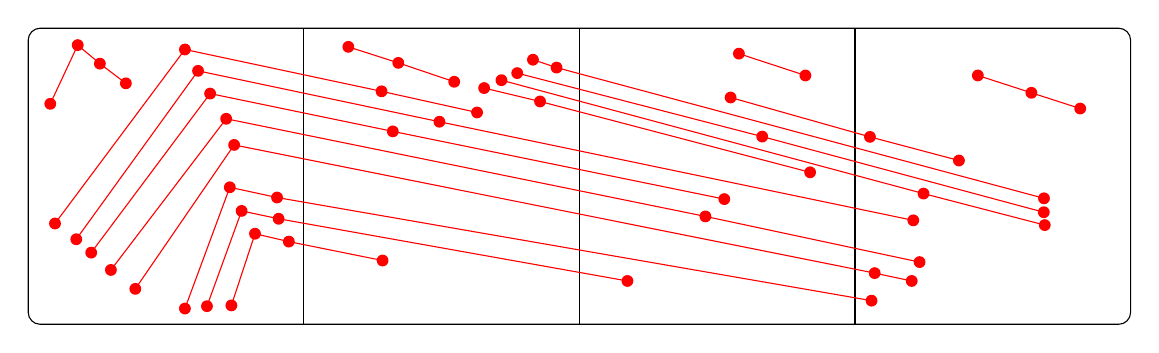
\begin{tikzpicture}[scale=1, every node/.style={scale=1}]
        \def\xscale{1.0} % Horizontal scale factor
        \def\yscale{1.0} % Vertical scale factor
        \def\spnt{0.075} % Size of smaller points
        \def\lpnt{0.125} % Size of larger points
        \def\roundscale{0.5} % The rounding factor
        \draw[rounded corners=2ex*\roundscale] (0,0) rectangle (14.0*\xscale,3.76*\yscale);
        \draw (3.5*\xscale, 3.76*\yscale) -- (3.5*\xscale, 0);
        \draw (7.0*\xscale, 3.76*\yscale) -- (7.0*\xscale, 0);
        \draw (10.5*\xscale, 3.76*\yscale) -- (10.5*\xscale, 0);
        \fill[red] (9.025415261218319*\xscale, 3.4370300409410106*\yscale) circle (\spnt);
        \fill[red] (9.87*\xscale, 3.16*\yscale) circle (\spnt);
        \draw[red] (9.025415261218319*\xscale, 3.4370300409410106*\yscale) -- (9.87*\xscale,3.16*\yscale);
        \fill[red] (4.065389790651616*\xscale, 3.523465393533877*\yscale) circle (\spnt);
        \fill[red] (4.7*\xscale, 3.32*\yscale) circle (\spnt);
        \fill[red] (5.41*\xscale, 3.08*\yscale) circle (\spnt);
        \draw[red] (4.065389790651616*\xscale, 3.523465393533877*\yscale) -- (4.7*\xscale,3.32*\yscale) -- (5.41*\xscale,3.08*\yscale);
        \fill[red] (5.79*\xscale, 3.0*\yscale) circle (\spnt);
        \fill[red] (6.5*\xscale, 2.83*\yscale) circle (\spnt);
        \fill[red] (9.93*\xscale, 1.93*\yscale) circle (\spnt);
        \draw[red] (5.79*\xscale, 3.0*\yscale) -- (6.5*\xscale,2.83*\yscale) -- (9.93*\xscale,1.93*\yscale);
        \fill[red] (6.41*\xscale, 3.36*\yscale) circle (\spnt);
        \fill[red] (6.71*\xscale, 3.26*\yscale) circle (\spnt);
        \fill[red] (12.9*\xscale, 1.6*\yscale) circle (\spnt);
        \draw[red] (6.41*\xscale, 3.36*\yscale) -- (6.71*\xscale,3.26*\yscale) -- (12.9*\xscale,1.6*\yscale);
        \fill[red] (6.21*\xscale, 3.19*\yscale) circle (\spnt);
        \fill[red] (9.32171125483173*\xscale, 2.383876554253752*\yscale) circle (\spnt);
        \fill[red] (12.897616736321888*\xscale, 1.4229999446867156*\yscale) circle (\spnt);
        \draw[red] (6.21*\xscale, 3.19*\yscale) -- (9.32171125483173*\xscale,2.383876554253752*\yscale) -- (12.897616736321888*\xscale,1.4229999446867156*\yscale);
        \fill[red] (6.01*\xscale, 3.1*\yscale) circle (\spnt);
        \fill[red] (11.37*\xscale, 1.66*\yscale) circle (\spnt);
        \fill[red] (12.91*\xscale, 1.26*\yscale) circle (\spnt);
        \draw[red] (6.01*\xscale, 3.1*\yscale) -- (11.37*\xscale,1.66*\yscale) -- (12.91*\xscale,1.26*\yscale);
        \fill[red] (8.92*\xscale, 2.88*\yscale) circle (\spnt);
        \fill[red] (10.69*\xscale, 2.38*\yscale) circle (\spnt);
        \fill[red] (11.82*\xscale, 2.08*\yscale) circle (\spnt);
        \draw[red] (8.92*\xscale, 2.88*\yscale) -- (10.69*\xscale,2.38*\yscale) -- (11.82*\xscale,2.08*\yscale);
        \fill[red] (12.06*\xscale, 3.16*\yscale) circle (\spnt);
        \fill[red] (12.74*\xscale, 2.94*\yscale) circle (\spnt);
        \fill[red] (13.36*\xscale, 2.74*\yscale) circle (\spnt);
        \draw[red] (12.06*\xscale, 3.16*\yscale) -- (12.74*\xscale,2.94*\yscale) -- (13.36*\xscale,2.74*\yscale);
        \fill[red] (0.28*\xscale, 2.8*\yscale) circle (\spnt);
        \fill[red] (0.6286433582040536*\xscale, 3.545653104388464*\yscale) circle (\spnt);
        \fill[red] (0.91*\xscale, 3.31*\yscale) circle (\spnt);
        \fill[red] (1.24*\xscale, 3.06*\yscale) circle (\spnt);
        \draw[red] (0.28*\xscale, 2.8*\yscale) -- (0.6286433582040536*\xscale,3.545653104388464*\yscale) -- (0.91*\xscale,3.31*\yscale) -- (1.24*\xscale,3.06*\yscale);
        \fill[red] (2.58*\xscale, 0.24*\yscale) circle (\spnt);
        \fill[red] (2.88*\xscale, 1.15*\yscale) circle (\spnt);
        \fill[red] (3.31*\xscale, 1.05*\yscale) circle (\spnt);
        \fill[red] (4.5*\xscale, 0.81*\yscale) circle (\spnt);
        \draw[red] (2.58*\xscale, 0.24*\yscale) -- (2.88*\xscale,1.15*\yscale) -- (3.31*\xscale,1.05*\yscale) -- (4.5*\xscale,0.81*\yscale);
        \fill[red] (2.27*\xscale, 0.23*\yscale) circle (\spnt);
        \fill[red] (2.71*\xscale, 1.44*\yscale) circle (\spnt);
        \fill[red] (3.18*\xscale, 1.34*\yscale) circle (\spnt);
        \fill[red] (7.61*\xscale, 0.55*\yscale) circle (\spnt);
        \draw[red] (2.27*\xscale, 0.23*\yscale) -- (2.71*\xscale,1.44*\yscale) -- (3.18*\xscale,1.34*\yscale) -- (7.61*\xscale,0.55*\yscale);
        \fill[red] (1.99*\xscale, 0.2*\yscale) circle (\spnt);
        \fill[red] (2.56*\xscale, 1.74*\yscale) circle (\spnt);
        \fill[red] (3.16*\xscale, 1.61*\yscale) circle (\spnt);
        \fill[red] (10.71*\xscale, 0.3*\yscale) circle (\spnt);
        \draw[red] (1.99*\xscale, 0.2*\yscale) -- (2.56*\xscale,1.74*\yscale) -- (3.16*\xscale,1.61*\yscale) -- (10.71*\xscale,0.3*\yscale);
        \fill[red] (0.34*\xscale, 1.28*\yscale) circle (\spnt);
        \fill[red] (1.99*\xscale, 3.49*\yscale) circle (\spnt);
        \fill[red] (4.487393024959084*\xscale, 2.958642977916958*\yscale) circle (\spnt);
        \fill[red] (5.7*\xscale, 2.69*\yscale) circle (\spnt);
        \draw[red] (0.34*\xscale, 1.28*\yscale) -- (1.99*\xscale,3.49*\yscale) -- (4.487393024959084*\xscale,2.958642977916958*\yscale) -- (5.7*\xscale,2.69*\yscale);
        \fill[red] (0.8*\xscale, 0.91*\yscale) circle (\spnt);
        \fill[red] (2.31*\xscale, 2.93*\yscale) circle (\spnt);
        \fill[red] (4.63*\xscale, 2.45*\yscale) circle (\spnt);
        \fill[red] (8.84*\xscale, 1.59*\yscale) circle (\spnt);
        \draw[red] (0.8*\xscale, 0.91*\yscale) -- (2.31*\xscale,2.93*\yscale) -- (4.63*\xscale,2.45*\yscale) -- (8.84*\xscale,1.59*\yscale);
        \fill[red] (0.61*\xscale, 1.08*\yscale) circle (\spnt);
        \fill[red] (2.1566952483766944*\xscale, 3.218645736093965*\yscale) circle (\spnt);
        \fill[red] (5.222205855724229*\xscale, 2.5723906205811886*\yscale) circle (\spnt);
        \fill[red] (11.24*\xscale, 1.32*\yscale) circle (\spnt);
        \draw[red] (0.61*\xscale, 1.08*\yscale) -- (2.1566952483766944*\xscale,3.218645736093965*\yscale) -- (5.222205855724229*\xscale,2.5723906205811886*\yscale) -- (11.24*\xscale,1.32*\yscale);
        \fill[red] (1.05*\xscale, 0.69*\yscale) circle (\spnt);
        \fill[red] (2.5140566365004244*\xscale, 2.6099847688049023*\yscale) circle (\spnt);
        \fill[red] (8.6*\xscale, 1.37*\yscale) circle (\spnt);
        \fill[red] (11.32*\xscale, 0.79*\yscale) circle (\spnt);
        \draw[red] (1.05*\xscale, 0.69*\yscale) -- (2.5140566365004244*\xscale,2.6099847688049023*\yscale) -- (8.6*\xscale,1.37*\yscale) -- (11.32*\xscale,0.79*\yscale);
        \fill[red] (1.36*\xscale, 0.45*\yscale) circle (\spnt);
        \fill[red] (2.6149931853267754*\xscale, 2.278050249126386*\yscale) circle (\spnt);
        \fill[red] (10.75*\xscale, 0.65*\yscale) circle (\spnt);
        \fill[red] (11.22*\xscale, 0.55*\yscale) circle (\spnt);
        \draw[red] (1.36*\xscale, 0.45*\yscale) -- (2.6149931853267754*\xscale,2.278050249126386*\yscale) -- (10.75*\xscale,0.65*\yscale) -- (11.22*\xscale,0.55*\yscale);
\end{tikzpicture}
\end{center}
\begin{center}
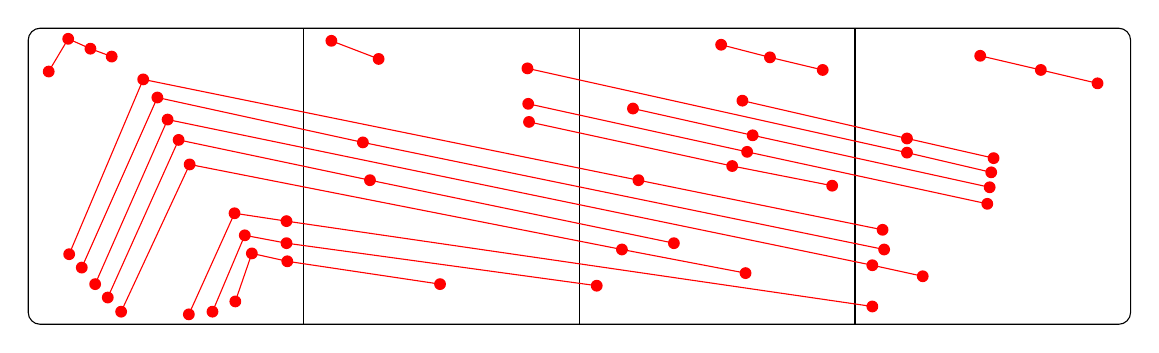
\begin{tikzpicture}[scale=1, every node/.style={scale=1}]
        \def\xscale{1.0} % Horizontal scale factor
        \def\yscale{1.0} % Vertical scale factor
        \def\spnt{0.075} % Size of smaller points
        \def\lpnt{0.125} % Size of larger points
        \def\roundscale{0.5} % The rounding factor
        \draw[rounded corners=2ex*\roundscale] (0,0) rectangle (14.0*\xscale,3.76*\yscale);
        \draw (3.5*\xscale, 3.76*\yscale) -- (3.5*\xscale, 0);
        \draw (7.0*\xscale, 3.76*\yscale) -- (7.0*\xscale, 0);
        \draw (10.5*\xscale, 3.76*\yscale) -- (10.5*\xscale, 0);
        \fill[red] (3.85*\xscale, 3.6*\yscale) circle (\spnt);
        \fill[red] (4.45*\xscale, 3.37*\yscale) circle (\spnt);
        \draw[red] (3.85*\xscale, 3.6*\yscale) -- (4.45*\xscale,3.37*\yscale);
        \fill[red] (6.36*\xscale, 2.57*\yscale) circle (\spnt);
        \fill[red] (8.94*\xscale, 2.01*\yscale) circle (\spnt);
        \fill[red] (10.21*\xscale, 1.76*\yscale) circle (\spnt);
        \draw[red] (6.36*\xscale, 2.57*\yscale) -- (8.94*\xscale,2.01*\yscale) -- (10.21*\xscale,1.76*\yscale);
        \fill[red] (6.35*\xscale, 2.8*\yscale) circle (\spnt);
        \fill[red] (9.13*\xscale, 2.19*\yscale) circle (\spnt);
        \fill[red] (12.18*\xscale, 1.53*\yscale) circle (\spnt);
        \draw[red] (6.35*\xscale, 2.8*\yscale) -- (9.13*\xscale,2.19*\yscale) -- (12.18*\xscale,1.53*\yscale);
        \fill[red] (6.34*\xscale, 3.25*\yscale) circle (\spnt);
        \fill[red] (11.16*\xscale, 2.18*\yscale) circle (\spnt);
        \fill[red] (12.23*\xscale, 1.93*\yscale) circle (\spnt);
        \draw[red] (6.34*\xscale, 3.25*\yscale) -- (11.16*\xscale,2.18*\yscale) -- (12.23*\xscale,1.93*\yscale);
        \fill[red] (8.8*\xscale, 3.55*\yscale) circle (\spnt);
        \fill[red] (9.42*\xscale, 3.39*\yscale) circle (\spnt);
        \fill[red] (10.09*\xscale, 3.23*\yscale) circle (\spnt);
        \draw[red] (8.8*\xscale, 3.55*\yscale) -- (9.42*\xscale,3.39*\yscale) -- (10.09*\xscale,3.23*\yscale);
        \fill[red] (7.68*\xscale, 2.74*\yscale) circle (\spnt);
        \fill[red] (9.2*\xscale, 2.4*\yscale) circle (\spnt);
        \fill[red] (12.21*\xscale, 1.74*\yscale) circle (\spnt);
        \draw[red] (7.68*\xscale, 2.74*\yscale) -- (9.2*\xscale,2.4*\yscale) -- (12.21*\xscale,1.74*\yscale);
        \fill[red] (9.07*\xscale, 2.84*\yscale) circle (\spnt);
        \fill[red] (11.16*\xscale, 2.36*\yscale) circle (\spnt);
        \fill[red] (12.26*\xscale, 2.11*\yscale) circle (\spnt);
        \draw[red] (9.07*\xscale, 2.84*\yscale) -- (11.16*\xscale,2.36*\yscale) -- (12.26*\xscale,2.11*\yscale);
        \fill[red] (12.09*\xscale, 3.41*\yscale) circle (\spnt);
        \fill[red] (12.86*\xscale, 3.23*\yscale) circle (\spnt);
        \fill[red] (13.58*\xscale, 3.06*\yscale) circle (\spnt);
        \draw[red] (12.09*\xscale, 3.41*\yscale) -- (12.86*\xscale,3.23*\yscale) -- (13.58*\xscale,3.06*\yscale);
        \fill[red] (0.26*\xscale, 3.21*\yscale) circle (\spnt);
        \fill[red] (0.5075971682687679*\xscale, 3.6255329896438315*\yscale) circle (\spnt);
        \fill[red] (0.79*\xscale, 3.5*\yscale) circle (\spnt);
        \fill[red] (1.06*\xscale, 3.4*\yscale) circle (\spnt);
        \draw[red] (0.26*\xscale, 3.21*\yscale) -- (0.5075971682687679*\xscale,3.6255329896438315*\yscale) -- (0.79*\xscale,3.5*\yscale) -- (1.06*\xscale,3.4*\yscale);
        \fill[red] (2.63*\xscale, 0.29*\yscale) circle (\spnt);
        \fill[red] (2.84*\xscale, 0.9*\yscale) circle (\spnt);
        \fill[red] (3.29*\xscale, 0.8*\yscale) circle (\spnt);
        \fill[red] (5.23*\xscale, 0.51*\yscale) circle (\spnt);
        \draw[red] (2.63*\xscale, 0.29*\yscale) -- (2.84*\xscale,0.9*\yscale) -- (3.29*\xscale,0.8*\yscale) -- (5.23*\xscale,0.51*\yscale);
        \fill[red] (2.34*\xscale, 0.16*\yscale) circle (\spnt);
        \fill[red] (2.75*\xscale, 1.13*\yscale) circle (\spnt);
        \fill[red] (3.28*\xscale, 1.03*\yscale) circle (\spnt);
        \fill[red] (7.22*\xscale, 0.49*\yscale) circle (\spnt);
        \draw[red] (2.34*\xscale, 0.16*\yscale) -- (2.75*\xscale,1.13*\yscale) -- (3.28*\xscale,1.03*\yscale) -- (7.22*\xscale,0.49*\yscale);
        \fill[red] (2.04*\xscale, 0.1261498920289589*\yscale) circle (\spnt);
        \fill[red] (2.62*\xscale, 1.41*\yscale) circle (\spnt);
        \fill[red] (3.28*\xscale, 1.31*\yscale) circle (\spnt);
        \fill[red] (10.72*\xscale, 0.2261498920289589*\yscale) circle (\spnt);
        \draw[red] (2.04*\xscale, 0.1261498920289589*\yscale) -- (2.62*\xscale,1.41*\yscale) -- (3.28*\xscale,1.31*\yscale) -- (10.72*\xscale,0.2261498920289589*\yscale);
        \fill[red] (1.01*\xscale, 0.34*\yscale) circle (\spnt);
        \fill[red] (1.91*\xscale, 2.3416773657739633*\yscale) circle (\spnt);
        \fill[red] (4.34*\xscale, 1.83*\yscale) circle (\spnt);
        \fill[red] (8.2*\xscale, 1.03*\yscale) circle (\spnt);
        \draw[red] (1.01*\xscale, 0.34*\yscale) -- (1.91*\xscale,2.3416773657739633*\yscale) -- (4.34*\xscale,1.83*\yscale) -- (8.2*\xscale,1.03*\yscale);
        \fill[red] (0.68*\xscale, 0.72*\yscale) circle (\spnt);
        \fill[red] (1.64*\xscale, 2.88*\yscale) circle (\spnt);
        \fill[red] (4.25*\xscale, 2.31*\yscale) circle (\spnt);
        \fill[red] (10.87*\xscale, 0.95*\yscale) circle (\spnt);
        \draw[red] (0.68*\xscale, 0.72*\yscale) -- (1.64*\xscale,2.88*\yscale) -- (4.25*\xscale,2.31*\yscale) -- (10.87*\xscale,0.95*\yscale);
        \fill[red] (1.18*\xscale, 0.16*\yscale) circle (\spnt);
        \fill[red] (2.05*\xscale, 2.03*\yscale) circle (\spnt);
        \fill[red] (7.54*\xscale, 0.95*\yscale) circle (\spnt);
        \fill[red] (9.11*\xscale, 0.65*\yscale) circle (\spnt);
        \draw[red] (1.18*\xscale, 0.16*\yscale) -- (2.05*\xscale,2.03*\yscale) -- (7.54*\xscale,0.95*\yscale) -- (9.11*\xscale,0.65*\yscale);
        \fill[red] (0.52*\xscale, 0.89*\yscale) circle (\spnt);
        \fill[red] (1.46*\xscale, 3.11*\yscale) circle (\spnt);
        \fill[red] (7.75*\xscale, 1.83*\yscale) circle (\spnt);
        \fill[red] (10.85*\xscale, 1.2*\yscale) circle (\spnt);
        \draw[red] (0.52*\xscale, 0.89*\yscale) -- (1.46*\xscale,3.11*\yscale) -- (7.75*\xscale,1.83*\yscale) -- (10.85*\xscale,1.2*\yscale);
        \fill[red] (0.85*\xscale, 0.51*\yscale) circle (\spnt);
        \fill[red] (1.77*\xscale, 2.6*\yscale) circle (\spnt);
        \fill[red] (10.72*\xscale, 0.75*\yscale) circle (\spnt);
        \fill[red] (11.36*\xscale, 0.61*\yscale) circle (\spnt);
        \draw[red] (0.85*\xscale, 0.51*\yscale) -- (1.77*\xscale,2.6*\yscale) -- (10.72*\xscale,0.75*\yscale) -- (11.36*\xscale,0.61*\yscale);
\end{tikzpicture}
\end{center}
    \caption{The pair of tilings that motivated the sliding strategy. The one above is the one encountered when mimicking the strategies of a specification for $\Av{1234}$ to a $\Av{1432}$ root while the one below is the one we needed to have identical specification in terms of strategies and structure.}
    \label{fig:slidepair}
\end{figure}

\section{Column reverse}
\begin{definition}\label{def:rrgp}
For a gridded permutation $\pi=\pi_1^{(x_1,y_1)}\pi_2^{(x_2,y_2)}\dotsm\pi_n^{(x_n,y_n)} \in \mathcal{G}_n$ define its \emph{column reverse} for $[a,b]$, where $a,b\in\N$ and $a\leq b$, as the mapping $\textsf{rev}_{[a,b]}$ where $\textsf{rev}_{[a,b]}(\pi)$ is $\pi$ where its longest subsequence whose columns all belong to interval
\[
\pi_{i}^{(x_i,y_i)}\pi_{i+1}^{(x_{i+1},y_{i+1})}\dotsm\pi_{i+k}^{(x_{i+k},y_{i+k})}
\]
has been replaced by 
\[
    \pi_{i+k}^{(a+b-x_{i+k},y_{i+k})}\dotsm\pi_{i+1}^{(a+b-x_{i+1},y_{i+1})}\pi_{i}^{(a+b-x_i,y_i)}.
\]
\end{definition}

The column reverse can be extended to subsequences of gridded permutations and tilings such that it is applied to all of its obstructions and requirements. Suppose $\pi = 5^{(0,1)}2^{(0,0)}4^{(1,1)}1^{(1,0)}6^{(2,2)}3^{(3,1)}$, then 
\[
\textsf{rev}_{[1,2]}(\pi) = 5^{(0,1)}2^{(0,0)}6^{(1,2)}1^{(2,0)}4^{(2,1)}3^{(3,1)},
\]
as shown in \FigureRef{fig:gp_col_rev}. An example for tilings can be seen in \FigureRef{fig:t_col_rev}.

\begin{figure}[htbp]
    \centering
    {
\newcommand{\picw}{1}
\newcommand{\pich}{1}
\begin{tikzpicture}
    \fill[gray!20] (\picw,0) rectangle (3*\picw,3*\pich);
    \draw (1 * \picw, 0) -- (1 * \picw, \pich * 3);
    \draw (2 * \picw, 0) -- (2 * \picw, \pich * 3);
    \draw (3 * \picw, 0) -- (3 * \picw, \pich * 3);
    \draw (0, 1 * \pich) -- (4 * \picw, 1 * \pich);
    \draw (0, 2 * \pich) -- (4 * \picw, 2 * \pich);
    \draw[rounded corners=2ex] (0,0) rectangle (4*\picw,3*\pich);
    \draw (0.25*\picw,3.5*0.5*\pich) -- (0.75*\picw,1*0.5*\pich) -- (1.25*\picw,3*0.5*\pich) -- (1.75*\picw,0.5*0.5*\pich) -- (2.5*\picw,5*0.5*\pich) -- (3.5*\picw,2.5*0.5*\pich);
    \fill (0.25*\picw,3.5*0.5*\pich) circle (0.075) node[below] {$5$};
    \fill (0.75*\picw,1*0.5*\pich) circle (0.075) node[below] {$2$};
    \fill (1.25*\picw,3*0.5*\pich) circle (0.075) node[above] {$4$};
    \fill (1.75*\picw,0.5*0.5*\pich) circle (0.075) node[left] {$1$};
    \fill (2.5*\picw,5*0.5*\pich) circle (0.075) node[above] {$6$};
    \fill (3.5*\picw,2.5*0.5*\pich) circle (0.075) node[above] {$3$};
\end{tikzpicture}
\begin{tikzpicture}
    \draw[white] (0,0) rectangle (2,3*\pich);
    \draw[thick, ->] (0.25,1.5*\pich) -- (1.75,1.5*\pich) node[above,pos=.5] {$\textsf{rev}_{[1,2]}$};
\end{tikzpicture}
\begin{tikzpicture}
    \fill[gray!20] (\picw,0) rectangle (3*\picw,3*\pich);
    \draw (1 * \picw, 0) -- (1 * \picw, \pich * 3);
    \draw (2 * \picw, 0) -- (2 * \picw, \pich * 3);
    \draw (3 * \picw, 0) -- (3 * \picw, \pich * 3);
    \draw (0, 1 * \pich) -- (4 * \picw, 1 * \pich);
    \draw (0, 2 * \pich) -- (4 * \picw, 2 * \pich);
    \draw[rounded corners=2ex] (0,0) rectangle (4*\picw,3*\pich);
    \draw (0.25*\picw,3.5*0.5*\pich) -- (0.75*\picw,1*0.5*\pich) -- (1.5*\picw,5*0.5*\pich) -- (2.25*\picw,0.5*0.5*\pich) -- (2.75*\picw,3*0.5*\pich) -- (3.5*\picw,2.5*0.5*\pich);
    \fill (0.25*\picw,3.5*0.5*\pich) circle (0.075) node[below] {$5$};
    \fill (0.75*\picw,1*0.5*\pich) circle (0.075) node[below] {$2$};
    \fill (1.5*\picw,5*0.5*\pich) circle (0.075) node[above] {$6$};
    \fill (2.25*\picw,0.5*0.5*\pich) circle (0.075) node[right] {$1$};
    \fill (2.75*\picw,3*0.5*\pich) circle (0.075) node[above] {$4$};
    \fill (3.5*\picw,2.5*0.5*\pich) circle (0.075) node[above] {$3$};
\end{tikzpicture}
}
    \caption{The column reverse of a gridded permutation.}
    \label{fig:gp_col_rev}
\end{figure}

\begin{figure}[htbp]
    \centering
    
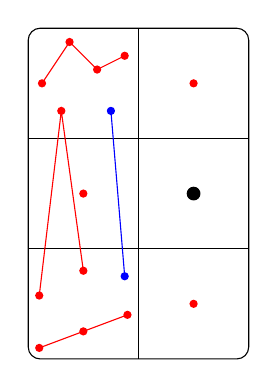
\begin{tikzpicture}[scale=0.7, every node/.style={scale=0.7}]
	\fill (3,3) circle (0.125);
	\fill[red] (1,3) circle (0.075);
	\fill[red] (3,5) circle (0.075);
	\fill[red] (3,1) circle (0.075);
    \draw[rounded corners=1ex] (0,0) rectangle (4,6);
    \draw (0,2) -- (4,2);
    \draw (0,4) -- (4,4);
    \draw (2,0) -- (2,6);
	\coordinate (a1) at (0.2,0.2);
	\coordinate (a2) at (1,0.5);
	\coordinate (a3) at (1.8,0.8);
	\coordinate (b1) at (0.2,1.15);
	\coordinate (b2) at (0.6,4.5);
	\coordinate (b3) at (1,1.6);
	\coordinate (c1) at (0.25,5);
	\coordinate (c2) at (0.75,5.75);
	\coordinate (c3) at (1.25,5.25);
	\coordinate (c4) at (1.75,5.5);
	\coordinate (d1) at (1.5,4.5);
	\coordinate (d2) at (1.75,1.5);
	\fill[red] (a1) circle (0.075);
	\fill[red] (a2) circle (0.075);
	\fill[red] (a3) circle (0.075);
	\fill[red] (b1) circle (0.075);
	\fill[red] (b2) circle (0.075);
	\fill[red] (b3) circle (0.075);
	\fill[red] (c1) circle (0.075);
	\fill[red] (c2) circle (0.075);
	\fill[red] (c3) circle (0.075);
	\fill[red] (c4) circle (0.075);
	\fill[blue] (d1) circle (0.075);
	\fill[blue] (d2) circle (0.075);
	\draw[red] (a1) -- (a2) -- (a3);
	\draw[red] (b1) -- (b2) -- (b3);
	\draw[red] (c1) -- (c2) -- (c3) -- (c4);
	\draw[blue] (d1) -- (d2);
\end{tikzpicture}
\begin{tikzpicture}[scale=0.7]
	\draw[white] (0,0) rectangle (2,6);
	\draw[thick, ->] (-.5,3) -- (2.5,3) node[above,pos=.5] {$\textsf{rev}_{[0,0]}$};
\end{tikzpicture}
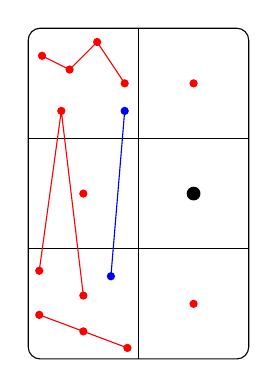
\begin{tikzpicture}[scale=0.7, every node/.style={scale=0.7}]
	\fill (3,3) circle (0.125);
	\fill[red] (1,3) circle (0.075);
	\fill[red] (3,5) circle (0.075);
	\fill[red] (3,1) circle (0.075);
    \draw[rounded corners=1ex] (0,0) rectangle (4,6);
    \draw (0,2) -- (4,2);
    \draw (0,4) -- (4,4);
    \draw (2,0) -- (2,6);
	\coordinate (a1) at (1.8,0.2);
	\coordinate (a2) at (1,0.5);
	\coordinate (a3) at (0.2,0.8);
	\coordinate (b1) at (1,1.15);
	\coordinate (b2) at (0.6,4.5);
	\coordinate (b3) at (0.2,1.6);
	\coordinate (c1) at (1.75,5);
	\coordinate (c2) at (1.25,5.75);
	\coordinate (c3) at (0.75,5.25);
	\coordinate (c4) at (0.25,5.5);
	\coordinate (d1) at (1.75,4.5);
	\coordinate (d2) at (1.5,1.5);
	\fill[red] (a1) circle (0.075);
	\fill[red] (a2) circle (0.075);
	\fill[red] (a3) circle (0.075);
	\fill[red] (b1) circle (0.075);
	\fill[red] (b2) circle (0.075);
	\fill[red] (b3) circle (0.075);
	\fill[red] (c1) circle (0.075);
	\fill[red] (c2) circle (0.075);
	\fill[red] (c3) circle (0.075);
	\fill[red] (c4) circle (0.075);
	\fill[blue] (d1) circle (0.075);
	\fill[blue] (d2) circle (0.075);
	\draw[red] (a1) -- (a2) -- (a3);
	\draw[red] (b1) -- (b2) -- (b3);
	\draw[red] (c1) -- (c2) -- (c3) -- (c4);
	\draw[blue] (d1) -- (d2);
\end{tikzpicture}
    \caption{The column reverse of a tiling.}
    \label{fig:t_col_rev}
\end{figure}

\begin{lemma}\label{lem:crevcontain}
Let $\pi, \sigma \in \mathcal{G}$ such that $\contains{\pi}{\sigma}$, then $\contains{\textsf{rev}_{[a,b]}(\pi)}{\textsf{rev}_{[a,b]}(\sigma)}$.
\end{lemma}
\begin{proof}
If $\pi$ has no elements within the columns then neither does $\sigma$ and both are mapped to themselves. If $\sigma$ has no elements within the columns then the mapping has no effect on the pattern which remains in $\textsf{rev}_{[a,b]}(\pi)$. 

Let $\set{i,i+1,\dotsc,i+k}$ be the indices of elements of $\pi$ with columns in $[a,b]$. Let $\sigma = \st{\sseq{A_1\cup L \cup A_2}{\pi}}$ where $L \subseteq \set{i,i+1,\dotsc,i+k}$ and $A_1$ and $A_2$ are the indices in $\pi$ on either side of the columns corresponding to the occurrence of $\sigma$, then
\begin{align*}
    \textsf{rev}_{[a,b]}(\sigma) &= \textsf{rev}_{[a,b]}\left(\st{\sseq{A_1\cup L \cup A_2}{\pi}}\right)\\ 
    &= \st{\textsf{rev}_{[a,b]}\left(\sseq{A_1\cup L \cup A_2}{\pi}\right)}\\
    &= \st{\textsf{rev}_{[a,b]}\left(\sseq{A_1}{\pi}\sseq{L}{\pi}\sseq{A_2}{\pi}\right)}\\
    &= \st{\sseq{A_1}{\pi}\textsf{rev}_{[a,b]}\left(\sseq{L}{\pi}\right)\sseq{A_2}{\pi}} \\
    &= \st{\sseq{A_1}{\textsf{rev}_{[a,b]}(\pi)}\textsf{rev}_{[a,b]}\left(\sseq{L}{\pi}\right)\sseq{A_2}{\textsf{rev}_{[a,b]}(\pi)}} \\
    &= \st{\sseq{A_1}{\textsf{rev}_{[a,b]}(\pi)}\sseq{\cset{2i+k-\ell}{\ell \in L}}{\textsf{rev}_{[a,b]}(\pi)}\sseq{A_2}{\textsf{rev}_{[a,b]}(\pi)}}\\
    &= \st{\sseq{A_1 \cup \cset{2i+k-\ell}{\ell \in L} \cup A_2}{\textsf{rev}_{[a,b]}(\pi)}}
\end{align*}
which shows that $\textsf{rev}_{[a,b]}(\sigma)$ is the standardization of a subsequence of $\textsf{rev}_{[a,b]}(\pi)$.
\end{proof}

%%%%%%%%%%%%%%%%%%%%%%%%%%%%%%%%%
% OLD WAY - split into lem&prop %
%%%%%%%%%%%%%%%%%%%%%%%%%%%%%%%%%
\begin{comment}
\begin{lemma}\label{lem:crevgrid}
Let $\mathcal{T}$ be a tiling and $\pi \in \textsf{Grid}(\mathcal{T})$, then $\textsf{rev}_{[a,b]}(\pi)\in\textsf{Grid}(\textsf{rev}_{[a,b]}(\mathcal{T}))$.
\end{lemma}
\begin{proof}
By Lemma \ref{lem:crevcontain} all occurrences of requirements are preserved so the only way that $\textsf{rev}_{[a,b]}(\pi)$ is not in $\textsf{Grid}(\textsf{rev}_{[a,b]}(\mathcal{T}))$ is if there exists an obstruction $o$ that is avoided by $\pi$ while $\textsf{rev}_{[a,b]}(\pi)$ contains $\textsf{rev}_{[a,b]}(o)$. Suppose that there is such an obstruction, then $\textsf{rev}_{[a,b]}(\textsf{rev}_{[a,b]}(\pi)) = \pi$ must contain $\textsf{rev}_{[a,b]}(\textsf{rev}_{[a,b]}(o)) = o$ which contradicts $\pi$ avoiding $o$.
\end{proof}

\begin{proposition}\label{prop:rrtil}
Let $\mathcal{T}$ be a tiling, then $|\textsf{Grid}_n(\mathcal{T})| = |\textsf{Grid}_n(\textsf{rev}_{[a,b]}(\mathcal{T}))|$ for all $n\in\N$.
\end{proposition}
\begin{proof}
With $\textsf{rev}_{[a,b]}$ being its own inverse it is a bijection between
\[
\textsf{Grid}_n(\mathcal{T}) \text{ and } \cset{\textsf{rev}_{[a,b]}(\pi)}{\pi \in \textsf{Grid}_n(\mathcal{T})}
\]
with the latter being a subset of $\textsf{Grid}_n(\textsf{rev}_{[a,b]}(\mathcal{T}))$ by Lemma \ref{lem:crevgrid} and therefore we have $|\textsf{Grid}_n(\mathcal{T})| \leq |\textsf{Grid}_n(\textsf{rev}_{[a,b]}(\mathcal{T}))|$. By the same argument there is a bijection between
\[
    \textsf{Grid}_n(\textsf{rev}_{[a,b]}(\mathcal{T})) \text{ and } \cset{\textsf{rev}_{[a,b]}(\pi)}{\pi \in \textsf{Grid}_n(\textsf{rev}_{[a,b]}(\mathcal{T}))}
\]
with the latter being a subset of $\textsf{Grid}_n(\textsf{rev}_{[a,b]}(\textsf{rev}_{[a,b]}(\mathcal{T})))=\textsf{Grid}_n(\mathcal{T})$ and therefore $|\textsf{Grid}_n(\mathcal{T})| \geq |\textsf{Grid}_n(\textsf{rev}_{[a,b]}(\mathcal{T}))|$ which shows that $|\textsf{Grid}_n(\mathcal{T})| = |\textsf{Grid}_n(\textsf{rev}_{[a,b]}(\mathcal{T}))|$.
\end{proof}
\end{comment}
%%%%%%%%%%%%%%%%%%
% END OF OLD WAY %
%%%%%%%%%%%%%%%%%%


%%%%%%%%%%%%%
%% New way %%
%%%%%%%%%%%%%
\begin{proposition}\label{prop:rrtil}
Let $\mathcal{T}$ be a tiling, then $|\textsf{Grid}_n(\mathcal{T})| = |\textsf{Grid}_n(\textsf{rev}_{[a,b]}(\mathcal{T}))|$ for all $n\in\N$.
\end{proposition}
\begin{proof}
By Lemma \ref{lem:crevcontain} all occurrences of requirements are preserved so the only way that $\textsf{rev}_{[a,b]}(\pi)$ is not in $\textsf{Grid}(\textsf{rev}_{[a,b]}(\mathcal{T}))$ is if there exists an obstruction $o$ that is avoided by $\pi$ while $\textsf{rev}_{[a,b]}(\pi)$ contains $\textsf{rev}_{[a,b]}(o)$. Suppose that there is such an obstruction, then $\textsf{rev}_{[a,b]}(\textsf{rev}_{[a,b]}(\pi)) = \pi$ must contain $\textsf{rev}_{[a,b]}(\textsf{rev}_{[a,b]}(o)) = o$ which contradicts $\pi$ avoiding $o$. Therefore $\pi \in \textsf{Grid}(\mathcal{T})$ implies $\textsf{rev}_{[a,b]}(\pi) \in \textsf{Grid}(\textsf{rev}_{[a,b]}(\mathcal{T}))$. With $\textsf{rev}_{[a,b]}$ being its own inverse it is a bijection between
\[
\textsf{Grid}_n(\mathcal{T}) \text{ and } \cset{\textsf{rev}_{[a,b]}(\pi)}{\pi \in \textsf{Grid}_n(\mathcal{T})} \subseteq \textsf{Grid}_n(\textsf{rev}_{[a,b]}(\mathcal{T}))
\]
and thus $|\textsf{Grid}_n(\mathcal{T})| \leq |\textsf{Grid}_n(\textsf{rev}_{[a,b]}(\mathcal{T}))|$. Analogously, in the other direction, we have $|\textsf{Grid}_n(\mathcal{T})| \geq |\textsf{Grid}_n(\textsf{rev}_{[a,b]}(\mathcal{T}))|$.
\end{proof}
\section{Column permutation}
Let $\pi=\pi_1^{(x_1,y_1)}\pi_2^{(x_2,y_2)}\dotsm\pi_n^{(x_n,y_n)} \in \mathcal{G}_n$ and define $\chi_x(\pi) = \pi_1^{(x,y_1)}\pi_2^{(x,y_2)}\dotsm\pi_n^{(x,y_n)}$ for $x\in\N$, e.g.,
\[
\chi_{1}\left(1^{(0,0)}3^{(2,3)}2^{(5,2)}\right) = 1^{(1,0)}3^{(1,3)}2^{(1,2)}.
\]
We extend this map to subsequences of gridded permutations.

\begin{definition}
Let $\pi = \pi_1^{(x_1,y_1)}\pi_2^{(x_2,y_2)}\dotsm\pi_n^{(x_n,y_n)} \in \mathcal{G}_n^{(c,r)}$ and $\sigma \in \mathcal{S}_k$ for $k \geq c$. The \emph{column permutation} $\sigma$ of $\pi$ is 
\[
    C_\sigma(\pi) = \chi_0(\sseq{A_{\sigma_1}}{\pi})\chi_1(\sseq{A_{\sigma_2}}{\pi}) \dotsm \chi_{k-1}(\sseq{A_{\sigma_k}}{\pi})
\]
where $A_i = \cset{j \in [n]}{x_j = i - 1}$ for $i \in [k]$ are the sets of indices in column $i$.
\end{definition}

Note that $A_1,A_2,\dotsc,A_k$ can include empty sets and $\sigma$ can be larger than the number of columns the gridded permutation spans, but not vice versa. We extend this definition to tilings such that it is applied to all of its obstructions and requirements. Let $\sigma = 4312$ and
\[
\pi = 6^{(0,1)}2^{(0,0)}5^{(1,1)}3^{(1,0)}8^{(1,2)}4^{(2,1)}7^{(3,2)}1^{(3,0)},
\]
then $A_1=\set{1,2}$, $A_2=\set{3,4,5}$, $A_3=\set{6}$, $A_4=\set{7,8}$ and we have
\begin{align*}
    C_\sigma(\pi) &= \chi_0\left(\sseq{A_{\sigma_1}}{\pi}\right)\chi_1\left(\sseq{A_{\sigma_2}}{\pi}\right)\chi_2\left(\sseq{A_{\sigma_3}}{\pi}\right) \chi_3\left(\sseq{A_{\sigma_{4}}}{\pi}\right) \\
    &= \chi_0\left(\sseq{A_{4}}{\pi}\right)\chi_1\left(\sseq{A_{3}}{\pi}\right)\chi_2\left(\sseq{A_{1}}{\pi}\right)\chi_3\left(\sseq{A_{2}}{\pi}\right) \\
    &= \chi_0\left(\sseq{{\set{7,8}}}{\pi}\right) \chi_1\left(\sseq{{\set{6}}}{\pi}\right)\chi_2\left(\sseq{{\set{1,2}}}{\pi}\right)\chi_3\left(\sseq{\set{3,4,5}}{\pi}\right) \\
    &= \chi_0\left(7^{(3,2)}1^{(3,0)}\right)\chi_1\left(4^{(2,1)}\right)\chi_2\left(6^{(0,1)}2^{(0,0)}\right)\chi_3\left(5^{(1,1)}3^{(1,0)}8^{(1,2)}\right) \\
    &= 7^{(0,2)}1^{(0,0)}4^{(1,1)}6^{(2,1)}2^{(2,0)}5^{(3,1)}3^{(3,0)}8^{(3,2)}
\end{align*}
as is shown in \FigureRef{fig:gp_col_perm}. An example for tilings can be seen in \FigureRef{fig:t_col_perm}.

\begin{figure}[H]
    \centering
    {
\newcommand{\myscale}{0.7}
\begin{tikzpicture}[scale=\myscale, every node/.style={scale=\myscale}]
    \draw[rounded corners=2ex] (0,0) rectangle (8,6);
    \foreach \x in {2,4,6} {
        \draw (\x,0) -- (\x,6);
    }
    \foreach \y in {2,4} {
        \draw (0,\y) -- (8, \y);
    }
    \draw (0.5,3.5) -- (1.5,1) -- (2.5,3) -- (3,1.5) -- (3.5,5.5) -- (5,2.5) -- (6.5,4.5) -- (7.5,.5);
    
    \fill (0.5,3.5) circle (0.1) node[above] {$6$};
    \fill (1.5,1) circle (0.1) node[below] {$2$};
    \fill (2.5,3) circle (0.1) node[above] {$5$};
    \fill (3,1.5) circle (0.1) node[below] {$3$};
    \fill (3.5,5.5) circle (0.1) node[above] {$8$};
    \fill (5,2.5) circle (0.1) node[below] {$4$};
    \fill (6.5,4.5) circle (0.1) node[above] {$7$};
    \fill (7.5,.5) circle (0.1) node[below] {$1$};
    \foreach \x in {1,2,3,4} {
        \draw (\x*2-1, 0) node[below] {$\x$};
    }
\end{tikzpicture}
\begin{tikzpicture}[scale=\myscale]
    \draw[white] (0,0) rectangle (2,6);
    \draw[thick, ->] (0,3.4) -- (2,3.4) node[above,pos=.5] {$C_{4312}$};
\end{tikzpicture}
\begin{tikzpicture}[scale=\myscale, every node/.style={scale=\myscale}]
    \draw[rounded corners=2ex] (0,0) rectangle (8,6);
    \foreach \x in {2,4,6} {
        \draw (\x,0) -- (\x,6);
    }
    \foreach \y in {2,4} {
        \draw (0,\y) -- (8, \y);
    }
    \draw (0.5,4.5) -- (1.5,.5) -- (3,2.5) -- (4.5,3.5) -- (5.5,1) -- (6.5,3) -- (7,1.5) -- (7.5,5.5);
    \fill (0.5,4.5) circle (0.1) node[above] {$7$};
    \fill (1.5,.5) circle (0.1) node[below] {$1$};
    \fill (3,2.5) circle (0.1) node[below] {$4$};
    \fill (4.5,3.5) circle (0.1) node[above] {$6$};
    \fill (5.5,1) circle (0.1) node[below] {$2$};
    \fill (6.5,3) circle (0.1) node[above] {$5$};
    \fill (7,1.5) circle (0.1) node[below] {$3$};
    \fill (7.5,5.5) circle (0.1) node[above] {$8$};
    \draw (1,0) node[below] {$4$};
    \draw (3,0) node[below] {$3$};
    \draw (5,0) node[below] {$1$};
    \draw (7,0) node[below] {$2$};
\end{tikzpicture}
}
    \caption{The column permutation of a gridded permutation.}
    \label{fig:gp_col_perm}
\end{figure}

\begin{figure}[!htbp]
    \centering
    {
\newcommand{\myscale}{0.75}
\begin{tikzpicture}[scale=\myscale, every node/.style={scale=\myscale}]
    \def\xscale{1.0} % Horizontal scale factor
    \def\yscale{0.95} % Vertical scale factor
    \def\spnt{0.075} % Size of smaller points
    \def\lpnt{0.125} % Size of larger points
    \draw[rounded corners=2ex] (0,0) rectangle (6*\xscale,6.26*\yscale);
    \fill[red] (5*\xscale,5.21666665*\yscale) circle (\spnt);
    \fill[red] (5*\xscale,3.13*\yscale) circle (\spnt);
    \fill[red] (3*\xscale,1.04333333*\yscale) circle (\spnt);
    \draw (2.0*\xscale, 6.26*\yscale) -- (2.0*\xscale, 0);
    \draw (4.0*\xscale, 6.26*\yscale) -- (4.0*\xscale, 0);
    \draw (0, 2.0866666666666664*\yscale) -- (6.0*\xscale, 2.0866666666666664*\yscale);
    \draw (0, 4.173333333333333*\yscale) -- (6.0*\xscale, 4.173333333333333*\yscale);
    \fill[red] (2.94*\xscale, 3.2*\yscale) circle (\spnt);
    \fill[red] (5.11*\xscale, 1.47*\yscale) circle (\spnt);
    \draw[red] (2.94*\xscale, 3.2*\yscale) -- (5.11*\xscale,1.47*\yscale);
    \fill[red] (4.498157727557963*\xscale, 1.1773727625023829*\yscale) circle (\spnt);
    \fill[red] (5.39*\xscale, 0.48*\yscale) circle (\spnt);
    \draw[red] (4.498157727557963*\xscale, 1.1773727625023829*\yscale) -- (5.39*\xscale,0.48*\yscale);
    \fill[red] (1.05*\xscale, 1.44*\yscale) circle (\spnt);
    \fill[red] (1.57*\xscale, 1.83*\yscale) circle (\spnt);
    \fill[red] (1.8507434638852711*\xscale, 3.256545283652403*\yscale) circle (\spnt);
    \draw[red] (1.05*\xscale, 1.44*\yscale) -- (1.57*\xscale,1.83*\yscale) -- (1.8507434638852711*\xscale,3.256545283652403*\yscale);
    \fill[red] (0.38*\xscale, 1.5*\yscale) circle (\spnt);
    \fill[red] (1.13*\xscale, 2.1866666666666665*\yscale) circle (\spnt);
    \fill[red] (1.36*\xscale, 2.85*\yscale) circle (\spnt);
    \draw[red] (0.38*\xscale, 1.5*\yscale) -- (1.13*\xscale,2.1866666666666665*\yscale) -- (1.36*\xscale,2.85*\yscale);
    \fill[red] (0.47*\xscale, 0.4256190749161856*\yscale) circle (\spnt);
    \fill[red] (0.99*\xscale, 1.08*\yscale) circle (\spnt);
    \fill[red] (1.53*\xscale, 0.74*\yscale) circle (\spnt);
    \draw[red] (0.47*\xscale, 0.4256190749161856*\yscale) -- (0.99*\xscale,1.08*\yscale) -- (1.53*\xscale,0.74*\yscale);
    \fill[red] (0.8*\xscale, 3.87*\yscale) circle (\spnt);
    \fill[red] (1.01*\xscale, 3.2095352654433555*\yscale) circle (\spnt);
    \fill[red] (1.59*\xscale, 3.5300000000000007*\yscale) circle (\spnt);
    \fill[red] (3.02*\xscale, 5.43*\yscale) circle (\spnt);
    \draw[red] (0.8*\xscale, 3.87*\yscale) -- (1.01*\xscale,3.2095352654433555*\yscale) -- (1.59*\xscale,3.5300000000000007*\yscale) -- (3.02*\xscale,5.43*\yscale);
    \fill[blue] (0.15*\xscale, 4.69*\yscale) circle (\spnt);
    \fill[blue] (0.56*\xscale, 1.97*\yscale) circle (\spnt);
    \draw[blue] (0.15*\xscale, 4.69*\yscale) -- (0.56*\xscale,1.97*\yscale);
\end{tikzpicture}
\begin{tikzpicture}
\draw[white] (0,0) rectangle (2,4);
\draw[thick, ->] (0.25,2.3) -- (1.75,2.3) node[above,pos=.5] {$C_{312}$};
\end{tikzpicture}
\begin{tikzpicture}[scale=\myscale, every node/.style={scale=\myscale}]
    \def\xscale{1.0} % Horizontal scale factor
    \def\yscale{0.95} % Vertical scale factor
    \def\spnt{0.075} % Size of smaller points
    \def\lpnt{0.125} % Size of larger points
    \draw[rounded corners=2ex] (0,0) rectangle (6*\xscale,6.26*\yscale);
    \fill[red] (1*\xscale, 5.21666667*\yscale) circle (\spnt);
    \fill[red] (1*\xscale, 3.13*\yscale) circle (\spnt);
    \fill[red] (5*\xscale, 1.04333333*\yscale) circle (\spnt);
    \draw (2.0*\xscale, 6.26*\yscale) -- (2.0*\xscale, 0);
    \draw (4.0*\xscale, 6.26*\yscale) -- (4.0*\xscale, 0);
    \draw (0, 2.0866666666666664*\yscale) -- (6.0*\xscale, 2.0866666666666664*\yscale);
    \draw (0, 4.173333333333333*\yscale) -- (6.0*\xscale, 4.173333333333333*\yscale);
    \fill[red] (1.71*\xscale, 0.21*\yscale) circle (\spnt);
    \fill[red] (5.32*\xscale, 2.93*\yscale) circle (\spnt);
    \draw[red] (1.71*\xscale, 0.21*\yscale) -- (5.32*\xscale,2.93*\yscale);
    \fill[red] (0.5850604532091456*\xscale, 1.4770759947591205*\yscale) circle (\spnt);
    \fill[red] (1.17*\xscale, 0.7*\yscale) circle (\spnt);
    \draw[red] (0.5850604532091456*\xscale, 1.4770759947591205*\yscale) -- (1.17*\xscale,0.7*\yscale);
    \fill[red] (2.28*\xscale, 1.16*\yscale) circle (\spnt);
    \fill[red] (3.13*\xscale, 1.65*\yscale) circle (\spnt);
    \fill[red] (3.63*\xscale, 2.48*\yscale) circle (\spnt);
    \draw[red] (2.28*\xscale, 1.16*\yscale) -- (3.13*\xscale,1.65*\yscale) -- (3.63*\xscale,2.48*\yscale);
    \fill[red] (2.57*\xscale, 1.69*\yscale) circle (\spnt);
    \fill[red] (2.85*\xscale, 2.59*\yscale) circle (\spnt);
    \fill[red] (3.62*\xscale, 3.1*\yscale) circle (\spnt);
    \draw[red] (2.57*\xscale, 1.69*\yscale) -- (2.85*\xscale,2.59*\yscale) -- (3.62*\xscale,3.1*\yscale);
    \fill[red] (3.01*\xscale, 0.26*\yscale) circle (\spnt);
    \fill[red] (3.34*\xscale, 1.07*\yscale) circle (\spnt);
    \fill[red] (3.68*\xscale, 0.73*\yscale) circle (\spnt);
    \draw[red] (3.01*\xscale, 0.26*\yscale) -- (3.34*\xscale,1.07*\yscale) -- (3.68*\xscale,0.73*\yscale);
    \fill[red] (2.56*\xscale, 3.88*\yscale) circle (\spnt);
    \fill[red] (2.91*\xscale, 3.13*\yscale) circle (\spnt);
    \fill[red] (3.48*\xscale, 3.58*\yscale) circle (\spnt);
    \fill[red] (5.11*\xscale, 5.3*\yscale) circle (\spnt);
    \draw[red] (2.56*\xscale, 3.88*\yscale) -- (2.91*\xscale,3.13*\yscale) -- (3.48*\xscale,3.58*\yscale) -- (5.11*\xscale,5.3*\yscale);
    \fill[blue] (2.1*\xscale, 4.91*\yscale) circle (\spnt);
    \fill[blue] (2.48*\xscale, 1.91*\yscale) circle (\spnt);
    \draw[blue] (2.1*\xscale, 4.91*\yscale) -- (2.48*\xscale,1.91*\yscale);
\end{tikzpicture}
}
    \caption{The column permutation of a tiling.}
    \label{fig:t_col_perm}
\end{figure}

Let $\pi=\pi_1\pi_2 \dotsm \pi_n \in\mathcal{S}_n$ and $A = (i_1, i_2,\dotsc,i_k)$ a finite sequence of size $k$ containing elements from $[n-1]$ and define the \emph{adjacent swap} of $\pi$ (relative to $A$) as
\[
\textsf{AdjSwap}_{A}(\pi) = \begin{cases}
\pi_1\pi_2 \dotsm \pi_{i_1-1}\pi_{i_1+1}\pi_{i_1}\pi_{i_1+2}\pi_{i_1+3} \dotsm \pi_n & \mbox{ if } k = 1,\\
\textsf{AdjSwap}_{(i_2,i_3,\dotsc,i_k)}\left(\textsf{AdjSwap}_{(i_1)}(\pi)\right) & \mbox{ otherwise.}
\end{cases}
\]
Let $\pi = 1423$, then $\textsf{AdjSwap}_{(1,2)}(\pi) = \textsf{AdjSwap}_{(2)}(4123) = 4213$.

\begin{lemma}\label{lem:swap}
Let $\pi = 12\dotsm n \in \textsf{Av}_n(21)$ then
\[
    \cset{\textsf{AdjSwap}_A(\pi)}{A \text{ is a finite sequence of elements from } [n-1]} = \mathcal{S}_n
\]
\end{lemma}
It is well known that permutation groups can be generated by adjacent swaps, see e.g., \cite{adjacentperm}.

% Proof commented out since not needed...
\begin{comment}\begin{proof}
Suppose we can generate $\mathcal{S}_{n-1}$ this way from the permutation in $\textsf{Av}_{n-1}(21)$ and let $\pi = \pi_1 \pi_2 \dotsm \pi_n \in \mathcal{S}_n$ with $\pi_j = n$. Let $A = (i_1,i_2,\dotsc,i_k)$ be the sequence of swaps that turns $12\dotsm (n-1)$ into $\pi_1 \pi_2 \dotsm \pi_{j-1}\pi_{j+1}\dotsm \pi_n \in \mathcal{S}_{n-1}$, then
\begin{align*}
    \textsf{AdjSwap}_{(i_1,i_2,\dotsc,i_k, n-1, n-2,\dotsc,j)}(12\dotsm n) = \pi
\end{align*}
and since this holds for a base case, it holds for all sizes $n\in\N$.
\end{proof}\end{comment}

\begin{proposition}
Let $\mathcal{T} = ((c,r),\mathcal{O},\{\mathcal{R}_1,\dotsc,\mathcal{R}_k\})$ be a tiling. For all $\sigma\in\mathcal{S}_c$ and $n\in\mathbb{N}$ we have $|\textsf{Grid}_n(\mathcal{T})| = |\textsf{Grid}_n\left(C_\sigma(\mathcal{T})\right)|$.
\end{proposition}
\begin{proof}
Swapping two adjacent columns $i$ and $i+1$ can be expressed as compositions of bijections, $\textsf{rev}_{[i,i]} \circ \textsf{rev}_{[i+1,i+1]} \circ \textsf{rev}_{[i,i+1]}$ and by Lemma \ref{lem:swap} we can produce any permutation of columns given adjacent swaps.
\end{proof}
\section{Sliding}
Sliding is a generalization (to the setting of tilings) of the sliding lemma described in \citeauthor{slide} \cite[Lemma 2.2]{slide}.

\begin{definition}
Let $\pi = \pi_1^{(x_1,0)}\pi_2^{(x_2,0)}\cdots\pi_n^{(x_n,0)} \in \mathcal{G}^{(c,1)}_n$. We define \emph{sliding} as the map $\Upsilon: \mathcal{G}^{(c,1)}_n \to \mathcal{G}^{(c,1)}_n$ defined as follows.
\begin{enumerate}[a)]
    \item If $\pi$ has no elements in $(1,0)$, we move whatever is in $(0,0)$ to $(1,0)$ and we are done.
    \item If $\pi$ has elements in $(1,0)$, we start by shifting all elements in $(2,0), (3,0), \dotsc, (c-1,0)$ one cell to the right and then we do the following until we have depleted the elements of $\pi$ in $(0,0)$:
    \begin{enumerate}[i.]
        \item If the rightmost element in $(0,0)$ is larger than all elements in $(1,0)$, we move the rightmost element of $(1,0)$ to $(2,0)$ as the leftmost element and then we move the rightmost element of $(0,0)$ to $(1,0)$ as the leftmost element.
        \item If the rightmost element in $(0,0)$ has a larger element in $(1,0)$, then we move the rightmost element of $(0,0)$ to the right of the smallest element in $(1,0)$ that is larger than it and that element is moved to be the leftmost element in $(2,0)$.
    \end{enumerate}
    Finally we shift all elements one cell to the left.
\end{enumerate}
\end{definition}

This mapping is outlined in Algorithm~\ref{alg:slidealg}\footnote{Every algorithm in this thesis is accompanied by a Python implementation that can be found in the appropriate repository at \texttt{\href{https://github.com/PermutaTriangle}{https://github.com/PermutaTriangle}}.}. An example for $3594^{(0,0)}62^{(1,0)}718^{(2,0)}$ can be seen in \FigureRef{fig:slide_gp_example}.

\begin{algorithm}
{
\setphaserulewidth{.7pt}

\begin{algorithmic}[1]
\Statex \textbf{Input}: A gridded permutation $\pi = \pi_1^{(x_1,0)}\pi_2^{(x_2,0)} \cdots \pi_n^{(x_n,0)} \in \mathcal{G}^{(m,1)}_n$.
\Statex \textbf{Output}: A gridded permutation in $\mathcal{G}_n^{(m,1)}$ with $(0,0)$ slid through $(1,0)$.
\Procedure{slide}{$\pi$}
    \If{$\cset{i}{x_i = 1} = \emptyset$}
        \State \Return{$\pi_1^{(x_1+1-\textsf{sign}(x_1),0)}\pi_2^{(x_2+1-\textsf{sign}(x_2),0)} \cdots \pi_n^{(x_n+1-\textsf{sign}(x_n),0)}$}
    \EndIf
    
    \For{$i \gets |\cset{j}{x_j < 2}| + 1, n$}
        \State $x_i \gets x_i + 1$
    \EndFor
    
    \While{$\cset{j}{x_j = 0} \neq \emptyset$}
        \State $i \gets \max\cset{j}{x_j = 0}$
        \State $A \gets \cset{j}{x_j = 1 \text{ and } \pi_j > \pi_i}$
        \State $k \gets |\cset{j}{x_j < 2}|$
        \If{$A = \emptyset$}
            \State $x_k \gets 2$
            \State $x_i \gets 1$
        \Else
            \State $j \gets \max(A)$
            \State $\alpha \gets \pi_i$
            \State $\beta \gets \pi_j$
            \For{$z\gets i, j-1$}
                \State $\pi_{z}^{(x_z,y_z)} \gets \pi_{z+1}^{(x_{z+1},y_{z+1})}$
            \EndFor
            \State $\pi_{j-1} \gets \alpha$
            \For{$z\gets j, k - 1$}
                \State $\pi_{z}^{(x_z,y_z)} \gets \pi_{z+1}^{(x_{z+1},y_{z+1})}$
            \EndFor
            \State $\pi_{k}^{(x_k,y_k)} \gets \beta^{(2,0)}$
        \EndIf
    \EndWhile
    \State \Return{$\pi_1^{(x_1 - 1,0)}\pi_2^{(x_2 - 1,0)}\cdots\pi_n^{(x_n - 1,0)}$}
\EndProcedure
\end{algorithmic}

}
\caption{The sliding algorithm}
\label{alg:slidealg}
\end{algorithm}

\begin{figure}[ht!]
    \centering
    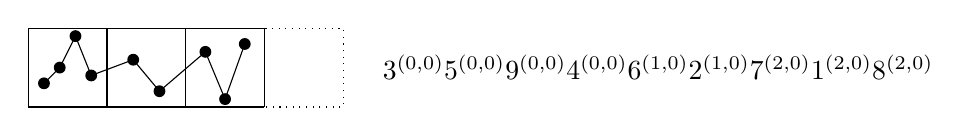
\begin{tikzpicture}
\def\xs{1.0}
\def\ys{1.0}
\def\ps{0.75}
\draw (0,0) grid[xscale=\xs,yscale=\ys] (3, 1);
\draw[dotted] (3*\xs,0) rectangle (4*\xs,1*\xs);
\coordinate (p0) at (0.2*\xs,0.30000000000000004*\ys);
\coordinate (p1) at (0.4*\xs,0.5*\ys);
\coordinate (p2) at (0.6000000000000001*\xs,0.9*\ys);
\coordinate (p3) at (0.8*\xs,0.4*\ys);
\coordinate (p4) at (1.3333333333333333*\xs,0.6000000000000001*\ys);
\coordinate (p5) at (1.6666666666666665*\xs,0.2*\ys);
\coordinate (p6) at (2.25*\xs,0.7000000000000001*\ys);
\coordinate (p7) at (2.5*\xs,0.1*\ys);
\coordinate (p8) at (2.75*\xs,0.8*\ys);
\draw (p0)--(p1)--(p2)--(p3)--(p4)--(p5)--(p6)--(p7)--(p8);
\fill (p0) circle (0.1*\ps);
\fill (p1) circle (0.1*\ps);
\fill (p2) circle (0.1*\ps);
\fill (p3) circle (0.1*\ps);
\fill (p4) circle (0.1*\ps);
\fill (p5) circle (0.1*\ps);
\fill (p6) circle (0.1*\ps);
\fill (p7) circle (0.1*\ps);
\fill (p8) circle (0.1*\ps);
\draw (8,0.5) node {$3^{(0,0)}5^{(0,0)}9^{(0,0)}4^{(0,0)}6^{(1,0)}2^{(1,0)}7^{(2,0)}1^{(2,0)}8^{(2,0)}$};
\end{tikzpicture}

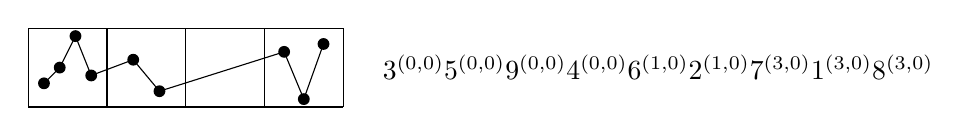
\begin{tikzpicture}
\def\xs{1.0}
\def\ys{1.0}
\def\ps{0.75}
\draw (0,0) grid[xscale=\xs,yscale=\ys] (4, 1);
\coordinate (p0) at (0.2*\xs,0.30000000000000004*\ys);
\coordinate (p1) at (0.4*\xs,0.5*\ys);
\coordinate (p2) at (0.6000000000000001*\xs,0.9*\ys);
\coordinate (p3) at (0.8*\xs,0.4*\ys);
\coordinate (p4) at (1.3333333333333333*\xs,0.6000000000000001*\ys);
\coordinate (p5) at (1.6666666666666665*\xs,0.2*\ys);
\coordinate (p6) at (1+2.25*\xs,0.7000000000000001*\ys);
\coordinate (p7) at (1+2.5*\xs,0.1*\ys);
\coordinate (p8) at (1+2.75*\xs,0.8*\ys);
\draw (p0)--(p1)--(p2)--(p3)--(p4)--(p5)--(p6)--(p7)--(p8);
\fill (p0) circle (0.1*\ps);
\fill (p1) circle (0.1*\ps);
\fill (p2) circle (0.1*\ps);
\fill (p3) circle (0.1*\ps);
\fill (p4) circle (0.1*\ps);
\fill (p5) circle (0.1*\ps);
\fill (p6) circle (0.1*\ps);
\fill (p7) circle (0.1*\ps);
\fill (p8) circle (0.1*\ps);
\draw (8,0.5) node {$3^{(0,0)}5^{(0,0)}9^{(0,0)}4^{(0,0)}6^{(1,0)}2^{(1,0)}7^{(3,0)}1^{(3,0)}8^{(3,0)}$};
\end{tikzpicture}

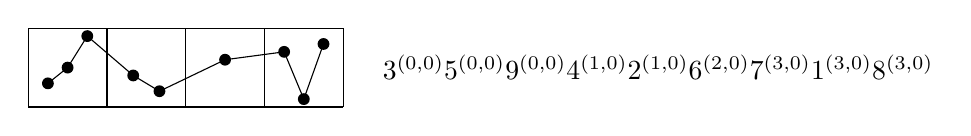
\begin{tikzpicture}
\def\xs{1.0}
\def\ys{1.0}
\def\ps{0.75}
\draw (0,0) grid[xscale=\xs,yscale=\ys] (4, 1);
\coordinate (p0) at (0.25*\xs,0.30000000000000004*\ys);
\coordinate (p1) at (0.5*\xs,0.5*\ys);
\coordinate (p2) at (0.75*\xs,0.9*\ys);
\coordinate (p3) at (1.3333333333333333*\xs,0.4*\ys);
\coordinate (p4) at (1.6666666666666665*\xs,0.2*\ys);
\coordinate (p5) at (2.5*\xs,0.6000000000000001*\ys);
\coordinate (p6) at (3.25*\xs,0.7000000000000001*\ys);
\coordinate (p7) at (3.5*\xs,0.1*\ys);
\coordinate (p8) at (3.75*\xs,0.8*\ys);
\draw (p0)--(p1)--(p2)--(p3)--(p4)--(p5)--(p6)--(p7)--(p8);
\fill (p0) circle (0.1*\ps);
\fill (p1) circle (0.1*\ps);
\fill (p2) circle (0.1*\ps);
\fill (p3) circle (0.1*\ps);
\fill (p4) circle (0.1*\ps);
\fill (p5) circle (0.1*\ps);
\fill (p6) circle (0.1*\ps);
\fill (p7) circle (0.1*\ps);
\fill (p8) circle (0.1*\ps);
\draw (8,0.5) node {$3^{(0,0)}5^{(0,0)}9^{(0,0)}4^{(1,0)}2^{(1,0)}6^{(2,0)}7^{(3,0)}1^{(3,0)}8^{(3,0)}$};
\end{tikzpicture}

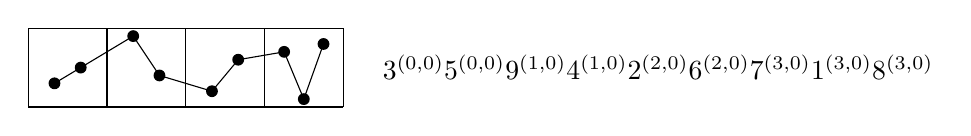
\begin{tikzpicture}
\def\xs{1.0}
\def\ys{1.0}
\def\ps{0.75}
\draw (0,0) grid[xscale=\xs,yscale=\ys] (4, 1);
\coordinate (p0) at (0.3333333333333333*\xs,0.30000000000000004*\ys);
\coordinate (p1) at (0.6666666666666666*\xs,0.5*\ys);
\coordinate (p2) at (1.3333333333333333*\xs,0.9*\ys);
\coordinate (p3) at (1.6666666666666665*\xs,0.4*\ys);
\coordinate (p4) at (2.3333333333333335*\xs,0.2*\ys);
\coordinate (p5) at (2.6666666666666665*\xs,0.6000000000000001*\ys);
\coordinate (p6) at (3.25*\xs,0.7000000000000001*\ys);
\coordinate (p7) at (3.5*\xs,0.1*\ys);
\coordinate (p8) at (3.75*\xs,0.8*\ys);
\draw (p0)--(p1)--(p2)--(p3)--(p4)--(p5)--(p6)--(p7)--(p8);
\fill (p0) circle (0.1*\ps);
\fill (p1) circle (0.1*\ps);
\fill (p2) circle (0.1*\ps);
\fill (p3) circle (0.1*\ps);
\fill (p4) circle (0.1*\ps);
\fill (p5) circle (0.1*\ps);
\fill (p6) circle (0.1*\ps);
\fill (p7) circle (0.1*\ps);
\fill (p8) circle (0.1*\ps);
\draw (8,0.5) node {$3^{(0,0)}5^{(0,0)}9^{(1,0)}4^{(1,0)}2^{(2,0)}6^{(2,0)}7^{(3,0)}1^{(3,0)}8^{(3,0)}$};
\end{tikzpicture}

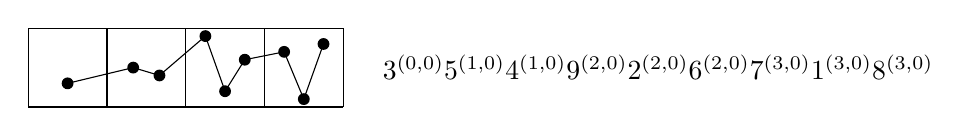
\begin{tikzpicture}
\def\xs{1.0}
\def\ys{1.0}
\def\ps{0.75}
\draw (0,0) grid[xscale=\xs,yscale=\ys] (4, 1);
\coordinate (p0) at (0.5*\xs,0.30000000000000004*\ys);
\coordinate (p1) at (1.3333333333333333*\xs,0.5*\ys);
\coordinate (p2) at (1.6666666666666665*\xs,0.4*\ys);
\coordinate (p3) at (2.25*\xs,0.9*\ys);
\coordinate (p4) at (2.5*\xs,0.2*\ys);
\coordinate (p5) at (2.75*\xs,0.6000000000000001*\ys);
\coordinate (p6) at (3.25*\xs,0.7000000000000001*\ys);
\coordinate (p7) at (3.5*\xs,0.1*\ys);
\coordinate (p8) at (3.75*\xs,0.8*\ys);
\draw (p0)--(p1)--(p2)--(p3)--(p4)--(p5)--(p6)--(p7)--(p8);
\fill (p0) circle (0.1*\ps);
\fill (p1) circle (0.1*\ps);
\fill (p2) circle (0.1*\ps);
\fill (p3) circle (0.1*\ps);
\fill (p4) circle (0.1*\ps);
\fill (p5) circle (0.1*\ps);
\fill (p6) circle (0.1*\ps);
\fill (p7) circle (0.1*\ps);
\fill (p8) circle (0.1*\ps);
\draw (8,0.5) node {$3^{(0,0)}5^{(1,0)}4^{(1,0)}9^{(2,0)}2^{(2,0)}6^{(2,0)}7^{(3,0)}1^{(3,0)}8^{(3,0)}$};
\end{tikzpicture}

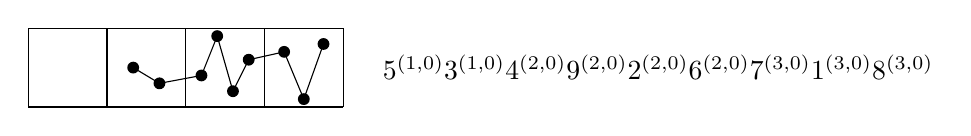
\begin{tikzpicture}
\def\xs{1.0}
\def\ys{1.0}
\def\ps{0.75}
\draw (0,0) grid[xscale=\xs,yscale=\ys] (4, 1);
\coordinate (p0) at (1.3333333333333333*\xs,0.5*\ys);
\coordinate (p1) at (1.6666666666666665*\xs,0.30000000000000004*\ys);
\coordinate (p2) at (2.2*\xs,0.4*\ys);
\coordinate (p3) at (2.4*\xs,0.9*\ys);
\coordinate (p4) at (2.6*\xs,0.2*\ys);
\coordinate (p5) at (2.8*\xs,0.6000000000000001*\ys);
\coordinate (p6) at (3.25*\xs,0.7000000000000001*\ys);
\coordinate (p7) at (3.5*\xs,0.1*\ys);
\coordinate (p8) at (3.75*\xs,0.8*\ys);
\draw (p0)--(p1)--(p2)--(p3)--(p4)--(p5)--(p6)--(p7)--(p8);
\fill (p0) circle (0.1*\ps);
\fill (p1) circle (0.1*\ps);
\fill (p2) circle (0.1*\ps);
\fill (p3) circle (0.1*\ps);
\fill (p4) circle (0.1*\ps);
\fill (p5) circle (0.1*\ps);
\fill (p6) circle (0.1*\ps);
\fill (p7) circle (0.1*\ps);
\fill (p8) circle (0.1*\ps);
\draw (8,0.5) node {$5^{(1,0)}3^{(1,0)}4^{(2,0)}9^{(2,0)}2^{(2,0)}6^{(2,0)}7^{(3,0)}1^{(3,0)}8^{(3,0)}$};
\end{tikzpicture}

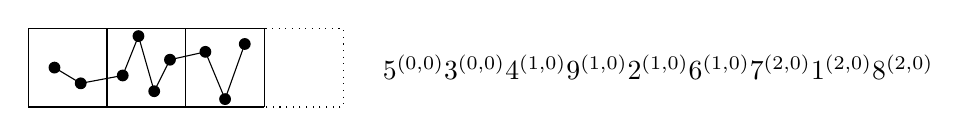
\begin{tikzpicture}
\def\xs{1.0}
\def\ys{1.0}
\def\ps{0.75}
\draw (0,0) grid[xscale=\xs,yscale=\ys] (3, 1);
\draw[dotted] (3*\xs,0) rectangle (4*\xs,1*\xs);
\coordinate (p0) at (-1+1.3333333333333333*\xs,0.5*\ys);
\coordinate (p1) at (-1+1.6666666666666665*\xs,0.30000000000000004*\ys);
\coordinate (p2) at (-1+2.2*\xs,0.4*\ys);
\coordinate (p3) at (-1+2.4*\xs,0.9*\ys);
\coordinate (p4) at (-1+2.6*\xs,0.2*\ys);
\coordinate (p5) at (-1+2.8*\xs,0.6000000000000001*\ys);
\coordinate (p6) at (-1+3.25*\xs,0.7000000000000001*\ys);
\coordinate (p7) at (-1+3.5*\xs,0.1*\ys);
\coordinate (p8) at (-1+3.75*\xs,0.8*\ys);
\draw (p0)--(p1)--(p2)--(p3)--(p4)--(p5)--(p6)--(p7)--(p8);
\fill (p0) circle (0.1*\ps);
\fill (p1) circle (0.1*\ps);
\fill (p2) circle (0.1*\ps);
\fill (p3) circle (0.1*\ps);
\fill (p4) circle (0.1*\ps);
\fill (p5) circle (0.1*\ps);
\fill (p6) circle (0.1*\ps);
\fill (p7) circle (0.1*\ps);
\fill (p8) circle (0.1*\ps);
\draw (8,0.5) node {$5^{(0,0)}3^{(0,0)}4^{(1,0)}9^{(1,0)}2^{(1,0)}6^{(1,0)}7^{(2,0)}1^{(2,0)}8^{(2,0)}$};
\end{tikzpicture}

\begin{tikzpicture}\end{tikzpicture}
    \caption{The sliding of $3594^{(0,0)}62^{(1,0)}718^{(2,0)}$.}
    \label{fig:slide_gp_example}
\end{figure}

\begin{definition}\label{def:slidable}
A pair of tilings
\[
    (\mathcal{T}_1,\mathcal{T}_2) = \left(\left((c,1), \mathcal{O}_1, \set{\mathcal{R}_1,\ldots,\mathcal{R}_k}\right), \left((c,1), \mathcal{O}_2, \set{\mathcal{R}'_1,\ldots,\mathcal{R}'_k}\right)\right)
\]
is \emph{slidable} if the following conditions are satisfied.
\begin{itemize}
    \item The tilings share requirements, that is $\set{\mathcal{R}_1,\ldots,\mathcal{R}_k}=\set{\mathcal{R}'_1,\ldots,\mathcal{R}'_k}$.
    \item No gridded permutation in $\mathcal{R}_1 \cup \cdots \cup \mathcal{R}_k$ has positions in columns $0$ and $1$.
    \item There exists an $n>1$ such that the obstructions $12\cdots n^{(0,0)}, 12\cdots (n-1)^{(0,0)}n^{(1,0)}$ and $12^{(1,0)}$ belong to $\mathcal{O}_1$, $12\cdots n^{(1,0)}, 1^{(0,0)}23\cdots n^{(1,0)}$ and $12^{(0,0)}$ belong to $\mathcal{O}_2$ and no other obstructions that are entirely within columns $0$ and $1$ belong to either $\mathcal{O}_1$ or $\mathcal{O}_2$.
    \item For any obstruction $\pi = \pi_1^{(x_1,0)}\pi_2^{(x_2,0)}\cdots\pi_n^{(x_w,0)} \in \mathcal{O}_1$ with at least one element outside columns $0$ and $1$ the subsequence $\sseq{\cset{i \in [w]}{x_i \in \set{0,1}}}{\pi}$ is either empty or in 
    \[
         \cset{j(j+1)^{(0,0)}, j^{(0,0)}(j+1)^{(1,0)}, j^{(0,0)},j^{(1,0)}}{j\in\Z^+}.
    \]
    Similarly, for $\mathcal{O}_2$, the subsequence must be either empty or in 
    \[
         \cset{j(j+1)^{(1,0)}, j^{(0,0)}(j+1)^{(1,0)}, j^{(0,0)},j^{(1,0)}}{j\in\Z^+}.
    \]
    \item Any obstruction entirely outside columns $0$ and $1$ in $\mathcal{O}_1$ must exist in $\mathcal{O}_2$ and vice versa.
    \item Let $o_1 = \pi_1^{(0,0)}\pi_2^{(x_2,0)}\cdots\pi_s^{(x_s,0)}$ and $o_2 = \pi_1^{(1,0)}\pi_2^{(x_2,0)}\cdots\pi_s^{(x_s,0)}$ where $x_2,s > 1$ then $o_1 \in \mathcal{O}_1$, $o_2 \in \mathcal{O}_1$, $o_1 \in \mathcal{O}_2$ and $o_2 \in \mathcal{O}_2$ are equivalent. That is, any crossing obstruction with one point in the first two columns must exist in both tilings and with that point in both columns.
    \item Let \begin{align*}o_1 &= \pi_1^{(0,0)}\pi_2^{(0,0)}\pi_3^{(x_3,0)}\cdots\pi_s^{(x_s,0)}\\o_2 &= \pi_1^{(0,0)}\pi_2^{(1,0)}\pi_3^{(x_3,0)}\cdots\pi_s^{(x_s,0)}\\o_3 &= \pi_1^{(1,0)}\pi_2^{(1,0)}\pi_3^{(x_3,0)}\cdots\pi_s^{(x_s,0)}\end{align*} where $s > 2$, $x_3 > 1$ and $\pi_1 + 1 = \pi_2$, then $o_1 \in \mathcal{O}_1$, $o_2 \in \mathcal{O}_1$, $o_2 \in \mathcal{O}_2$ and $o_3 \in \mathcal{O}_2$ are equivalent. That is, any crossing obstruction with $j(j+1)$ in the first two columns (and at least one point outside of those columns) must exists in both tilings where $j(j+1)$ has been spread between the first two columns in all possible ways, excluding the one that collides with the $12$ obstruction.
\end{itemize}
\end{definition}

An example of two slidable tilings can be seen in \FigureRef{fig:slidable_tilings}.

\begin{figure}[ht]
    \centering
    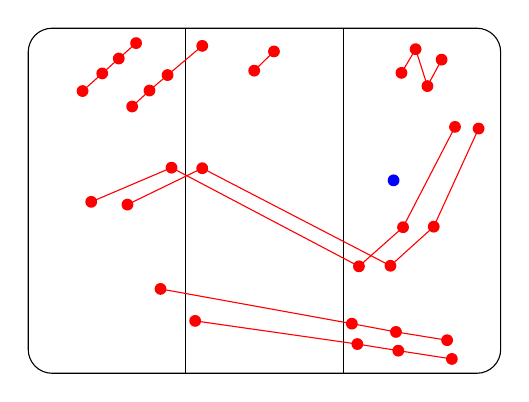
\begin{tikzpicture}[scale=1, every node/.style={scale=1}]
\def\xscale{1.0} % Horizontal scale factor
\def\yscale{0.7} % Vertical scale factor
\def\spnt{0.075} % Size of smaller points
\def\lpnt{0.125} % Size of larger points
\draw[rounded corners=2ex] (0,0) rectangle (6*\xscale,6.26*\yscale);
\draw (2.0*\xscale, 6.26*\yscale) -- (2.0*\xscale, 0);
\draw (4.0*\xscale, 6.26*\yscale) -- (4.0*\xscale, 0);
\fill[red] (2.87*\xscale, 5.49*\yscale) circle (\spnt);
\fill[red] (3.1209520279019056*\xscale, 5.838779282906702*\yscale) circle (\spnt);
\draw[red] (2.87*\xscale, 5.49*\yscale) -- (3.1209520279019056*\xscale,5.838779282906702*\yscale);
\fill[red] (0.69*\xscale, 5.12*\yscale) circle (\spnt);
\fill[red] (0.94*\xscale, 5.44*\yscale) circle (\spnt);
\fill[red] (1.15*\xscale, 5.71*\yscale) circle (\spnt);
\fill[red] (1.37*\xscale, 5.99*\yscale) circle (\spnt);
\draw[red] (0.69*\xscale, 5.12*\yscale) -- (0.94*\xscale,5.44*\yscale) -- (1.15*\xscale,5.71*\yscale) -- (1.37*\xscale,5.99*\yscale);
\fill[red] (1.32*\xscale, 4.84*\yscale) circle (\spnt);
\fill[red] (1.54*\xscale, 5.13*\yscale) circle (\spnt);
\fill[red] (1.77*\xscale, 5.41*\yscale) circle (\spnt);
\fill[red] (2.21*\xscale, 5.94*\yscale) circle (\spnt);
\draw[red] (1.32*\xscale, 4.84*\yscale) -- (1.54*\xscale,5.13*\yscale) -- (1.77*\xscale,5.41*\yscale) -- (2.21*\xscale,5.94*\yscale);
\fill[red] (4.74*\xscale, 5.45*\yscale) circle (\spnt);
\fill[red] (4.92*\xscale, 5.88*\yscale) circle (\spnt);
\fill[red] (5.07*\xscale, 5.21*\yscale) circle (\spnt);
\fill[red] (5.25*\xscale, 5.69*\yscale) circle (\spnt);
\draw[red] (4.74*\xscale, 5.45*\yscale) -- (4.92*\xscale,5.88*\yscale) -- (5.07*\xscale,5.21*\yscale) -- (5.25*\xscale,5.69*\yscale);
\fill[red] (1.68*\xscale, 1.53*\yscale) circle (\spnt);
\fill[red] (4.11*\xscale, 0.9*\yscale) circle (\spnt);
\fill[red] (4.67*\xscale, 0.75*\yscale) circle (\spnt);
\fill[red] (5.32*\xscale, 0.6*\yscale) circle (\spnt);
\draw[red] (1.68*\xscale, 1.53*\yscale) -- (4.11*\xscale,0.9*\yscale) -- (4.67*\xscale,0.75*\yscale) -- (5.32*\xscale,0.6*\yscale);
\fill[red] (2.12*\xscale, 0.95*\yscale) circle (\spnt);
\fill[red] (4.18*\xscale, 0.53*\yscale) circle (\spnt);
\fill[red] (4.7*\xscale, 0.41*\yscale) circle (\spnt);
\fill[red] (5.38*\xscale, 0.26*\yscale) circle (\spnt);
\draw[red] (2.12*\xscale, 0.95*\yscale) -- (4.18*\xscale,0.53*\yscale) -- (4.7*\xscale,0.41*\yscale) -- (5.38*\xscale,0.26*\yscale);
\fill[red] (0.8*\xscale, 3.11*\yscale) circle (\spnt);
\fill[red] (1.82*\xscale, 3.73*\yscale) circle (\spnt);
\fill[red] (4.2*\xscale, 1.94*\yscale) circle (\spnt);
\fill[red] (4.76*\xscale, 2.65*\yscale) circle (\spnt);
\fill[red] (5.42*\xscale, 4.47*\yscale) circle (\spnt);
\draw[red] (0.8*\xscale, 3.11*\yscale) -- (1.82*\xscale,3.73*\yscale) -- (4.2*\xscale,1.94*\yscale) -- (4.76*\xscale,2.65*\yscale) -- (5.42*\xscale,4.47*\yscale);
\fill[red] (1.26*\xscale, 3.06*\yscale) circle (\spnt);
\fill[red] (2.21*\xscale, 3.72*\yscale) circle (\spnt);
\fill[red] (4.6*\xscale, 1.95*\yscale) circle (\spnt);
\fill[red] (5.15*\xscale, 2.66*\yscale) circle (\spnt);
\fill[red] (5.72*\xscale, 4.44*\yscale) circle (\spnt);
\draw[red] (1.26*\xscale, 3.06*\yscale) -- (2.21*\xscale,3.72*\yscale) -- (4.6*\xscale,1.95*\yscale) -- (5.15*\xscale,2.66*\yscale) -- (5.72*\xscale,4.44*\yscale);
\fill[blue] (4.64*\xscale, 3.5*\yscale) circle (\spnt);
\end{tikzpicture}
\hspace{0.5cm}
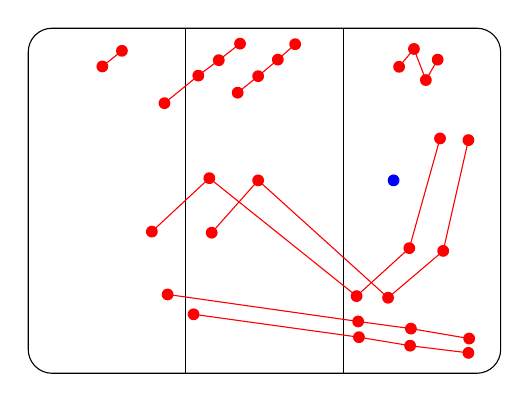
\begin{tikzpicture}[scale=1, every node/.style={scale=1}]
\def\xscale{1.0} % Horizontal scale factor
\def\yscale{0.7} % Vertical scale factor
\def\spnt{0.075} % Size of smaller points
\def\lpnt{0.125} % Size of larger points
\draw[rounded corners=2ex] (0,0) rectangle (6*\xscale,6.26*\yscale);
\draw (2.0*\xscale, 6.26*\yscale) -- (2.0*\xscale, 0);
\draw (4.0*\xscale, 6.26*\yscale) -- (4.0*\xscale, 0);
\fill[red] (0.9413254253242579*\xscale, 5.5665123438541855*\yscale) circle (\spnt);
\fill[red] (1.19*\xscale, 5.85*\yscale) circle (\spnt);
\draw[red] (0.9413254253242579*\xscale, 5.5665123438541855*\yscale) -- (1.19*\xscale,5.85*\yscale);
\fill[red] (1.73*\xscale, 4.9*\yscale) circle (\spnt);
\fill[red] (2.16*\xscale, 5.4*\yscale) circle (\spnt);
\fill[red] (2.42*\xscale, 5.68*\yscale) circle (\spnt);
\fill[red] (2.69*\xscale, 5.98*\yscale) circle (\spnt);
\draw[red] (1.73*\xscale, 4.9*\yscale) -- (2.16*\xscale,5.4*\yscale) -- (2.42*\xscale,5.68*\yscale) -- (2.69*\xscale,5.98*\yscale);
\fill[red] (2.66*\xscale, 5.09*\yscale) circle (\spnt);
\fill[red] (2.92*\xscale, 5.39*\yscale) circle (\spnt);
\fill[red] (3.17*\xscale, 5.69*\yscale) circle (\spnt);
\fill[red] (3.39*\xscale, 5.97*\yscale) circle (\spnt);
\draw[red] (2.66*\xscale, 5.09*\yscale) -- (2.92*\xscale,5.39*\yscale) -- (3.17*\xscale,5.69*\yscale) -- (3.39*\xscale,5.97*\yscale);
\fill[red] (4.71*\xscale, 5.56*\yscale) circle (\spnt);
\fill[red] (4.898395663501238*\xscale, 5.884152285333065*\yscale) circle (\spnt);
\fill[red] (5.05*\xscale, 5.32*\yscale) circle (\spnt);
\fill[red] (5.2*\xscale, 5.69*\yscale) circle (\spnt);
\draw[red] (4.71*\xscale, 5.56*\yscale) -- (4.898395663501238*\xscale,5.884152285333065*\yscale) -- (5.05*\xscale,5.32*\yscale) -- (5.2*\xscale,5.69*\yscale);
\fill[red] (1.77*\xscale, 1.43*\yscale) circle (\spnt);
\fill[red] (4.19*\xscale, 0.94*\yscale) circle (\spnt);
\fill[red] (4.86*\xscale, 0.81*\yscale) circle (\spnt);
\fill[red] (5.6*\xscale, 0.63*\yscale) circle (\spnt);
\draw[red] (1.77*\xscale, 1.43*\yscale) -- (4.19*\xscale,0.94*\yscale) -- (4.86*\xscale,0.81*\yscale) -- (5.6*\xscale,0.63*\yscale);
\fill[red] (2.1*\xscale, 1.07*\yscale) circle (\spnt);
\fill[red] (4.2*\xscale, 0.6546404918137944*\yscale) circle (\spnt);
\fill[red] (4.85*\xscale, 0.5*\yscale) circle (\spnt);
\fill[red] (5.59*\xscale, 0.37*\yscale) circle (\spnt);
\draw[red] (2.1*\xscale, 1.07*\yscale) -- (4.2*\xscale,0.6546404918137944*\yscale) -- (4.85*\xscale,0.5*\yscale) -- (5.59*\xscale,0.37*\yscale);
\fill[red] (1.57*\xscale, 2.57*\yscale) circle (\spnt);
\fill[red] (2.3*\xscale, 3.54*\yscale) circle (\spnt);
\fill[red] (4.17*\xscale, 1.4*\yscale) circle (\spnt);
\fill[red] (4.84*\xscale, 2.27*\yscale) circle (\spnt);
\fill[red] (5.23*\xscale, 4.26*\yscale) circle (\spnt);
\draw[red] (1.57*\xscale, 2.57*\yscale) -- (2.3*\xscale,3.54*\yscale) -- (4.17*\xscale,1.4*\yscale) -- (4.84*\xscale,2.27*\yscale) -- (5.23*\xscale,4.26*\yscale);
\fill[red] (2.33*\xscale, 2.55*\yscale) circle (\spnt);
\fill[red] (2.92*\xscale, 3.5*\yscale) circle (\spnt);
\fill[red] (4.57*\xscale, 1.37*\yscale) circle (\spnt);
\fill[red] (5.27*\xscale, 2.22*\yscale) circle (\spnt);
\fill[red] (5.59*\xscale, 4.23*\yscale) circle (\spnt);
\draw[red] (2.33*\xscale, 2.55*\yscale) -- (2.92*\xscale,3.5*\yscale) -- (4.57*\xscale,1.37*\yscale) -- (5.27*\xscale,2.22*\yscale) -- (5.59*\xscale,4.23*\yscale);
\fill[blue] (4.64*\xscale, 3.5*\yscale) circle (\spnt);
\end{tikzpicture}
    \caption{Typical slidable tilings.}
    \label{fig:slidable_tilings}
\end{figure}

\begin{lemma}\label{lem:slidemap}
Let $(\mathcal{T}_1,\mathcal{T}_2)$ be slidable and $i \in \N$, then $\Upsilon(\pi) \in \textsf{Grid}_i(\mathcal{T}_2)$ for every $\pi \in \textsf{Grid}_i(\mathcal{T}_1)$.
\end{lemma}
\begin{proof}
If $\pi$ contains no elements within the first two columns it is mapped to itself and since the tilings share requirements and are identical outside the first two columns then $\Upsilon(\pi) \in \textsf{Grid}_i(\mathcal{T}_2)$. If $\pi$ contains no elements in column $1$ then whatever is in column $0$ is moved to column $1$. Since $\pi$ avoided $12\dotsm n$ in column $0$ then $\Upsilon(\pi)$ will avoid $12\dotsm n$ in column $1$ and any crossing obstruction in $\mathcal{T}_2$ with one or two points in column $1$ would have existed with those points in column $0$ in $\mathcal{T}_1$ and therefore $\Upsilon(\pi) \in \textsf{Grid}_i(\mathcal{T}_2)$.

Now suppose $\pi$ has elements in column $1$. By the end of the mapping all columns are shifted one to the left but we will refer to their indices before the shift in the mapped tiling. Note that the mapping is defined by placing elements in-order into column $1$ so we will never form an increasing pattern there. 

Suppose after a single step in the map that we form the first $12\cdots n$ (spread in any way across the first $3$ columns). Note that it can contain at most one point in column $1$ as that column is decreasing.

If the $12\cdots n$ pattern does contain the newly moved point in column $1$ and not the one we moved to column $2$, then the pattern must have been there before the step was taken.

\begin{center}
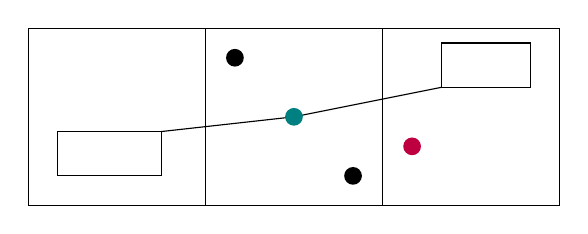
\begin{tikzpicture}[scale=0.75]
    \draw (2.25,1.25) -- (4.5,1.5) -- (7,2);
    \draw (0,0) rectangle (3,3);
    \draw (3,0) rectangle (6,3);
    \draw (6,0) rectangle (9,3);
    \fill (3.5,2.5) circle (0.15);
    \fill[teal] (4.5,1.5) circle (0.15);
    \fill (5.5,0.5) circle (0.15);
    \draw (0.5,0.5) rectangle (2.25,1.25);
    \fill[purple] (6.5,1) circle (0.15);
    \draw (7,2) rectangle (8.5,2.75);
\end{tikzpicture}
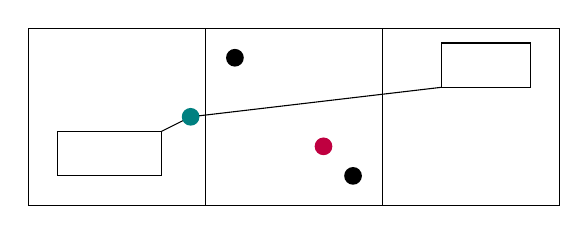
\begin{tikzpicture}[scale=0.75]
    \draw (2.25,1.25) -- (2.75,1.5) -- (7,2);
    \draw (0,0) rectangle (3,3);
    \draw (3,0) rectangle (6,3);
    \draw (6,0) rectangle (9,3);
    \fill (3.5,2.5) circle (0.15);
    \fill[teal] (2.75,1.5) circle (0.15);
    \fill (5.5,0.5) circle (0.15);
    \draw (0.5,0.5) rectangle (2.25,1.25);
    \fill[purple] (5,1) circle (0.15);
    \draw (7,2) rectangle (8.5,2.75);
\end{tikzpicture}
\end{center}

Suppose this pattern includes the newly moved element in column $2$ and no elements in column $1$ then the pattern must have existed before regardless of whether the new element in column $2$ was the smallest element in column $1$ before the move or not.

\begin{center}
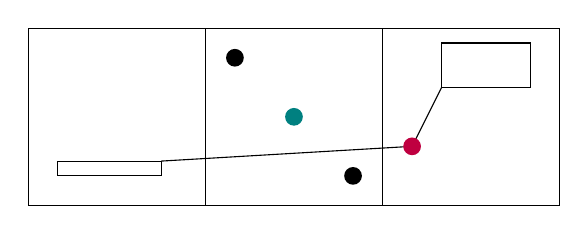
\begin{tikzpicture}[scale=0.75]
    \draw (2.25,0.75) -- (6.5,1) -- (7,2);
    \draw (0,0) rectangle (3,3);
    \draw (3,0) rectangle (6,3);
    \draw (6,0) rectangle (9,3);
    \fill (3.5,2.5) circle (0.15);
    \fill[teal] (4.5,1.5) circle (0.15);
    \fill (5.5,0.5) circle (0.15);
    \draw (0.5,0.5) rectangle (2.25,0.75);
    \fill[purple] (6.5,1) circle (0.15);
    \draw (7,2) rectangle (8.5,2.75);
\end{tikzpicture}
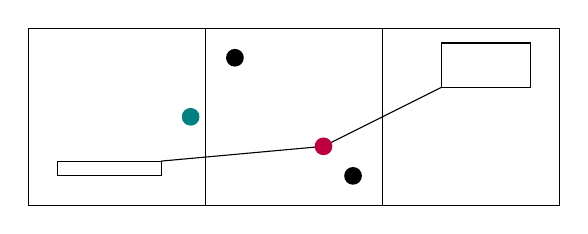
\begin{tikzpicture}[scale=0.75]
    \draw (2.25,0.75) -- (5,1) -- (7,2);
    \draw (0,0) rectangle (3,3);
    \draw (3,0) rectangle (6,3);
    \draw (6,0) rectangle (9,3);
    \fill (3.5,2.5) circle (0.15);
    \fill[teal] (2.75,1.5) circle (0.15);
    \fill (5.5,0.5) circle (0.15);
    \draw (0.5,0.5) rectangle (2.25,0.75);
    \fill[purple] (5,1) circle (0.15);
    \draw (7,2) rectangle (8.5,2.75);
\end{tikzpicture}
\end{center}

Finally suppose the pattern involves elements from both columns $1$ and $2$. Here two scenario can arise. One were the pattern involves both moved elements and the other only the one moved to column $2$. In the first one the pattern remains as we move both points together when we backtrack.

\begin{center}
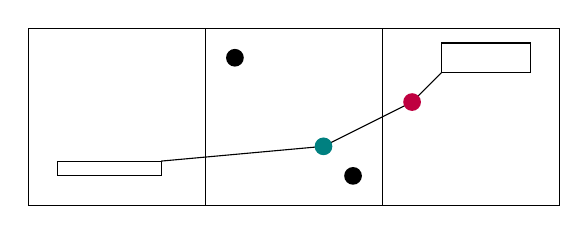
\begin{tikzpicture}[scale=0.75]
    \draw (2.25,0.75) -- (5,1) -- (6.5,1.75) -- (7,2.25);
    \draw (0,0) rectangle (3,3);
    \draw (3,0) rectangle (6,3);
    \draw (6,0) rectangle (9,3);
    \fill (3.5,2.5) circle (0.15);
    \fill[teal] (5,1) circle (0.15);
    \fill (5.5,0.5) circle (0.15);
    \draw (0.5,0.5) rectangle (2.25,0.75);
    \fill[purple] (6.5,1.75) circle (0.15);
    \draw (7,2.25) rectangle (8.5,2.75);
\end{tikzpicture}
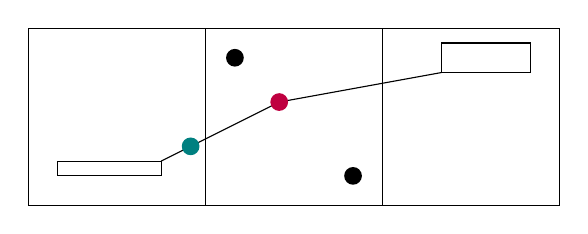
\begin{tikzpicture}[scale=0.75]
    \draw (2.25,0.75) -- (2.75,1) -- (4.25,1.75) -- (7,2.25);
    \draw (0,0) rectangle (3,3);
    \draw (3,0) rectangle (6,3);
    \draw (6,0) rectangle (9,3);
    \fill (3.5,2.5) circle (0.15);
    \fill[teal] (2.75,1) circle (0.15);
    \fill (5.5,0.5) circle (0.15);
    \draw (0.5,0.5) rectangle (2.25,0.75);
    \fill[purple] (4.25,1.75) circle (0.15);
    \draw (7,2.25) rectangle (8.5,2.75);
\end{tikzpicture}
\end{center}

In the latter, there is a smaller element in column $1$ than the moved one that belongs to the pattern. When we go back, the moved element goes back from column $1$ to column $0$ but that is between the element in column $1$ that formed the pattern and the element that was moved to column $2$, preserving the pattern.

\begin{center}
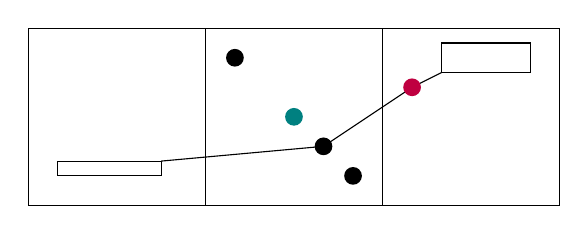
\begin{tikzpicture}[scale=0.75]
    \draw (2.25,0.75) -- (5,1) -- (6.5,2) -- (7,2.25);
    \draw (0,0) rectangle (3,3);
    \draw (3,0) rectangle (6,3);
    \draw (6,0) rectangle (9,3);
    \fill (5.5,0.5) circle (0.15);
    \fill (5,1) circle (0.15);
    \fill[teal] (4.5,1.5) circle (0.15);
    \fill[purple] (6.5,2) circle (0.15);
    \fill (3.5,2.5) circle (0.15);
    \draw (0.5,0.5) rectangle (2.25,0.75);
    \draw (7,2.25) rectangle (8.5,2.75);
\end{tikzpicture}
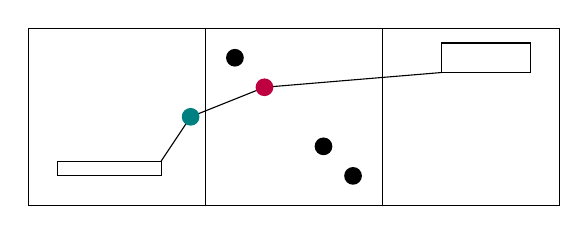
\begin{tikzpicture}[scale=0.75]
    \draw (2.25,0.75) -- (2.75,1.5) -- (4,2) -- (7,2.25);
    \draw (0,0) rectangle (3,3);
    \draw (3,0) rectangle (6,3);
    \draw (6,0) rectangle (9,3);
    \fill (5.5,0.5) circle (0.15);
    \fill (5,1) circle (0.15);
    \fill[teal] (2.75,1.5) circle (0.15);
    \fill[purple] (4,2) circle (0.15);
    \fill (3.5,2.5) circle (0.15);
    \draw (0.5,0.5) rectangle (2.25,0.75);
    \draw (7,2.25) rectangle (8.5,2.75);
\end{tikzpicture}
\end{center}

In the case of the first crossing obstructions forming for the first time with one element in the first 3 columns and some outside, then wherever that element was before must have been an occurrence of that pattern as well.

Now suppose we form the crossing pattern with the elements $k(k+1)$ in the first three columns (spread in any way) for the first time. This can happen in several ways. Note that the two increasing elements can not both be in column $1$ as it is always decreasing.

Suppose the $k(k+1)$ part in the first $3$ columns occurs between the first two, then the pattern must have existed before with $k(k+1)$ in column $0$.

\begin{center}
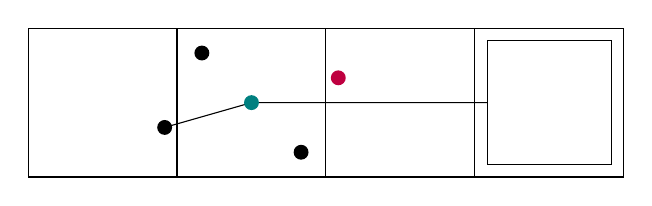
\begin{tikzpicture}[scale=0.63]
    \coordinate (a1) at (5.5,0.5);
    \coordinate (a2) at (2.75,1);
    \coordinate (a3) at (4.5,1.5);
    \coordinate (a4) at (6.25,2);
    \coordinate (a5) at (3.5,2.5);
    \draw (a2) -- (a3) -- (9.25,1.5);
    \draw (0,0) rectangle (3,3);
    \draw (3,0) rectangle (6,3);
    \draw (6,0) rectangle (9,3);
    \draw (9,0) rectangle (12,3);
    \fill (a1) circle (0.15);
    \fill (a2) circle (0.15);
    \fill[teal] (a3) circle (0.15);
    \fill[purple] (a4) circle (0.15);
    \fill (a5) circle (0.15);
    \draw (9.25,0.25) rectangle (11.75,2.75);
\end{tikzpicture}
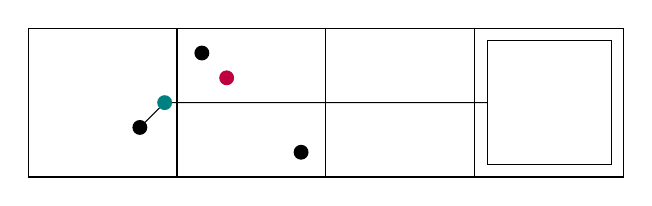
\begin{tikzpicture}[scale=0.63]
    \coordinate (a1) at (5.5,0.5);
    \coordinate (a2) at (2.25,1);
    \coordinate (a3) at (2.75,1.5);
    \coordinate (a4) at (4,2);
    \coordinate (a5) at (3.5,2.5);
    \draw (a2) -- (a3) -- (9.25,1.5);
    \draw (0,0) rectangle (3,3);
    \draw (3,0) rectangle (6,3);
    \draw (6,0) rectangle (9,3);
    \draw (9,0) rectangle (12,3);
    \fill (a1) circle (0.15);
    \fill (a2) circle (0.15);
    \fill[teal] (a3) circle (0.15);
    \fill[purple] (a4) circle (0.15);
    \fill (a5) circle (0.15);
    \draw (9.25,0.25) rectangle (11.75,2.75);
\end{tikzpicture}
\end{center}

If the pattern occurs with $k(k+1)$ in columns $0$ and $2$, then it must have existed with $k(k+1)$ in columns $0$ and $1$ before.

\begin{center}
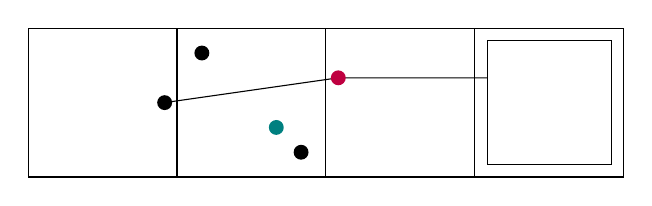
\begin{tikzpicture}[scale=0.63]
    \coordinate (a1) at (5.5,0.5);
    \coordinate (a2) at (5,1);
    \coordinate (a3) at (2.75,1.5);
    \coordinate (a4) at (6.25,2);
    \coordinate (a5) at (3.5,2.5);
    \draw (a3) -- (a4) -- (9.25,2);
    \draw (0,0) rectangle (3,3);
    \draw (3,0) rectangle (6,3);
    \draw (6,0) rectangle (9,3);
    \draw (9,0) rectangle (12,3);
    \fill (a1) circle (0.15);
    \fill[teal] (a2) circle (0.15);
    \fill (a3) circle (0.15);
    \fill[purple] (a4) circle (0.15);
    \fill (a5) circle (0.15);
    \draw (9.25,0.25) rectangle (11.75,2.75);
\end{tikzpicture}
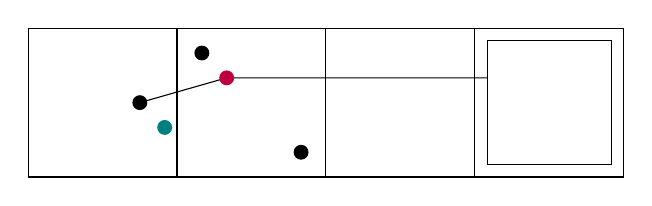
\begin{tikzpicture}[scale=0.63]
    \coordinate (a1) at (5.5,0.5);
    \coordinate (a2) at (2.75,1);
    \coordinate (a3) at (2.25,1.5);
    \coordinate (a4) at (4,2);
    \coordinate (a5) at (3.5,2.5);
    \draw (a3) -- (a4) -- (9.25,2);
    \draw (0,0) rectangle (3,3);
    \draw (3,0) rectangle (6,3);
    \draw (6,0) rectangle (9,3);
    \draw (9,0) rectangle (12,3);
    \fill (a1) circle (0.15);
    \fill[teal] (a2) circle (0.15);
    \fill (a3) circle (0.15);
    \fill[purple] (a4) circle (0.15);
    \fill (a5) circle (0.15);
    \draw (9.25,0.25) rectangle (11.75,2.75);
\end{tikzpicture}
\end{center}

If the pattern occurs with $k(k+1)$ in columns $1$ and $2$ they must be the two elements that were moved since they are adjacent in value and increasing and therefore the pattern must have existed with $k(k+1)$ in columns $0$ and $1$ before.

\begin{center}
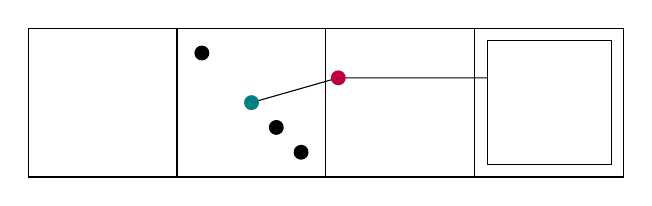
\begin{tikzpicture}[scale=0.63]
    \coordinate (a1) at (5.5,0.5);
    \coordinate (a2) at (5,1);
    \coordinate (a3) at (4.5,1.5);
    \coordinate (a4) at (6.25,2);
    \coordinate (a5) at (3.5,2.5);
    \draw (a3) -- (a4) -- (9.25,2);
    \draw (0,0) rectangle (3,3);
    \draw (3,0) rectangle (6,3);
    \draw (6,0) rectangle (9,3);
    \draw (9,0) rectangle (12,3);
    \fill (a1) circle (0.15);
    \fill (a2) circle (0.15);
    \fill[teal] (a3) circle (0.15);
    \fill[purple] (a4) circle (0.15);
    \fill (a5) circle (0.15);
    \draw (9.25,0.25) rectangle (11.75,2.75);
\end{tikzpicture}
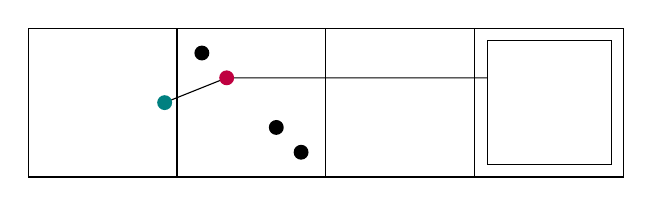
\begin{tikzpicture}[scale=0.63]
    \coordinate (a1) at (5.5,0.5);
    \coordinate (a2) at (5,1);
    \coordinate (a3) at (2.75,1.5);
    \coordinate (a4) at (4,2);
    \coordinate (a5) at (3.5,2.5);
    \draw (a3) -- (a4) -- (9.25,2);
    \draw (0,0) rectangle (3,3);
    \draw (3,0) rectangle (6,3);
    \draw (6,0) rectangle (9,3);
    \draw (9,0) rectangle (12,3);
    \fill (a1) circle (0.15);
    \fill (a2) circle (0.15);
    \fill[teal] (a3) circle (0.15);
    \fill[purple] (a4) circle (0.15);
    \fill (a5) circle (0.15);
    \draw (9.25,0.25) rectangle (11.75,2.75);
\end{tikzpicture}
\end{center}

If the pattern occurs with $k(k+1)$ entirely within column $2$, then the pattern must have existed with $k(k+1)$ in columns $1$ and $2$ before.

\begin{center}
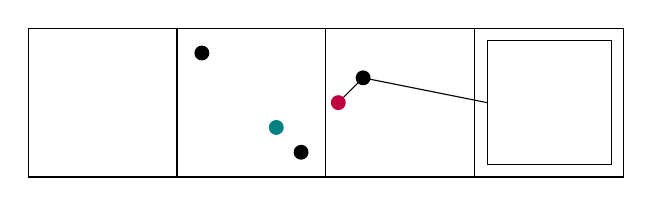
\begin{tikzpicture}[scale=0.63]
    \coordinate (a1) at (5.5,0.5);
    \coordinate (a2) at (5,1);
    \coordinate (a3) at (6.25,1.5);
    \coordinate (a4) at (6.75,2);
    \coordinate (a5) at (3.5,2.5);
    \draw (a3) -- (a4) -- (9.25,1.5);
    \draw (0,0) rectangle (3,3);
    \draw (3,0) rectangle (6,3);
    \draw (6,0) rectangle (9,3);
    \draw (9,0) rectangle (12,3);
    \fill (a1) circle (0.15);
    \fill[teal] (a2) circle (0.15);
    \fill[purple] (a3) circle (0.15);
    \fill (a4) circle (0.15);
    \fill (a5) circle (0.15);
    \draw (9.25,0.25) rectangle (11.75,2.75);
\end{tikzpicture}
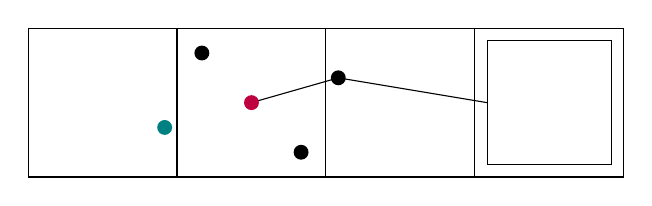
\begin{tikzpicture}[scale=0.63]
    \coordinate (a1) at (5.5,0.5);
    \coordinate (a2) at (2.75,1);
    \coordinate (a3) at (4.5,1.5);
    \coordinate (a4) at (6.25,2);
    \coordinate (a5) at (3.5,2.5);
    \draw (a3) -- (a4) -- (9.25,1.5);
    \draw (0,0) rectangle (3,3);
    \draw (3,0) rectangle (6,3);
    \draw (6,0) rectangle (9,3);
    \draw (9,0) rectangle (12,3);
    \fill (a1) circle (0.15);
    \fill[teal] (a2) circle (0.15);
    \fill[purple] (a3) circle (0.15);
    \fill (a4) circle (0.15);
    \fill (a5) circle (0.15);
    \draw (9.25,0.25) rectangle (11.75,2.75);
\end{tikzpicture}
\end{center}

The trivial bijection of shifting the entire gridded permutation one column to the left (with column $0$ being depleted after the mapping) will not create any of these patterns. Since no obstruction from $\mathcal{T}_2$ can occur, $\Upsilon(\pi)$ is in $\textsf{Grid}_i(\mathcal{T}_2)$.
\end{proof}

\begin{definition}
Let $\pi = \pi_1^{(x_1,0)}\pi_2^{(x_2,0)}\cdots\pi_n^{(x_n,0)} \in \mathcal{G}^{(c,1)}_n$. We define \emph{inverse sliding} as the map $\Upsilon^{-1}: \mathcal{G}^{(c,1)}_n \to \mathcal{G}^{(c,1)}_n$ defined as follows.
\begin{enumerate}[a)]
    \item If $\pi$ has no elements in $(0,0)$, we move whatever is in $(1,0)$ to $(0,0)$ and we are done.
    \item If $\pi$ has elements in $(0,0)$, we start by shifting all elements one cell to the right and then we do the following until we have depleted the elements of $\pi$ in $(2,0)$:
    \begin{enumerate}[i.]
        \item If the leftmost element in $(2,0)$ is smaller than all elements in $(1,0)$, we move the leftmost element of $(1,0)$ to $(0,0)$ as the rightmost element and then we move the leftmost element of $(2,0)$ to $(1,0)$ as the rightmost element.
        \item If the leftmost element in $(2,0)$ has a smaller element in $(1,0)$, then we move the leftmost element in $(2,0)$ to the left of the largest element in $(1,0)$ that is smaller than it and that element is moved to be the rightmost element in $(0,0)$.
    \end{enumerate}
    Finally we shift all elements in $(3,0), (4,0), \ldots$ one cell to the left.
\end{enumerate}
\end{definition}

\begin{lemma}
Let $(\mathcal{T}_1,\mathcal{T}_2)$ be slidable and $i \in \N$, then $\Upsilon^{-1}(\pi) \in \textsf{Grid}_i(\mathcal{T}_1)$ for every $\pi \in \textsf{Grid}_i(\mathcal{T}_2)$.
\end{lemma}
\begin{proof}
The argument when $(0,0)$ is empty is an analog of the case in Lemma \ref{lem:slidemap} when $(1,0)$ is empty so we assume that $\pi$ has elements in $(0,0)$. The avoidance of $12\cdots n$ and any crossing obstruction is an analog of the same case in Lemma \ref{lem:slidemap}, viewing the images from right to left instead.
\end{proof}

\begin{proposition}
Let $(\mathcal{T}_1,\mathcal{T}_2)$ be slidable, then $|\textsf{Grid}_i(\mathcal{T}_1)| = |\textsf{Grid}_i(\mathcal{T}_2)|$ for all $i\in\N$.
\end{proposition}
\begin{proof}
Let $\pi \in \textsf{Grid}_i(\mathcal{T}_1)$ and $\pi' \in \textsf{Grid}_i(\mathcal{T}_2)$. A step in $\Upsilon$ where we move an element larger than all the elements in $(1,0)$ is cancelled out by the corresponding move in $\Upsilon^{-1}$ and vice versa.

\begin{center}
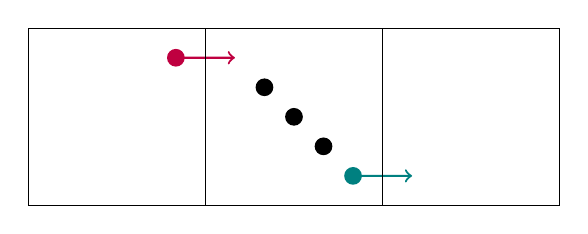
\begin{tikzpicture}[scale=0.75]
    \coordinate (a1) at (5.5,0.5);
    \coordinate (a2) at (5,1);
    \coordinate (a3) at (4.5,1.5);
    \coordinate (a4) at (4,2);
    \coordinate (a5) at (2.5,2.5);
    \draw[purple,->,thick] (a5) -- (3.5,2.5);
    \draw[teal,->,thick] (a1) -- (6.5,0.5);
    \draw (0,0) rectangle (3,3);
    \draw (3,0) rectangle (6,3);
    \draw (6,0) rectangle (9,3);
    \fill[teal] (a1) circle (0.15);
    \fill (a2) circle (0.15);
    \fill (a3) circle (0.15);
    \fill (a4) circle (0.15);
    \fill[purple] (a5) circle (0.15);
\end{tikzpicture}
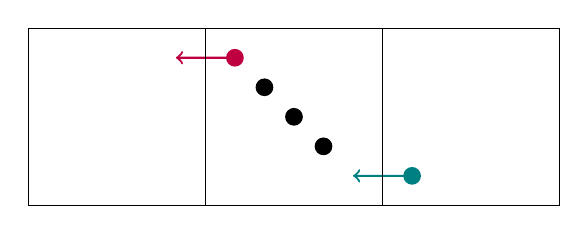
\begin{tikzpicture}[scale=0.75]
    \coordinate (a1) at (6.5,0.5);
    \coordinate (a2) at (5,1);
    \coordinate (a3) at (4.5,1.5);
    \coordinate (a4) at (4,2);
    \coordinate (a5) at (3.5,2.5);
    \draw[purple,->,thick] (a5) -- (2.5,2.5);
    \draw[teal,->,thick] (a1) -- (5.5,0.5);
    \draw (0,0) rectangle (3,3);
    \draw (3,0) rectangle (6,3);
    \draw (6,0) rectangle (9,3);
    \fill[teal] (a1) circle (0.15);
    \fill (a2) circle (0.15);
    \fill (a3) circle (0.15);
    \fill (a4) circle (0.15);
    \fill[purple] (a5) circle (0.15);
\end{tikzpicture}
\end{center}

A step in $\Upsilon$ where we move an element not larger than all elements in $(1,0)$ is cancelled out by the corresponding move in $\Upsilon^{-1}$ and vice versa.

\begin{center}
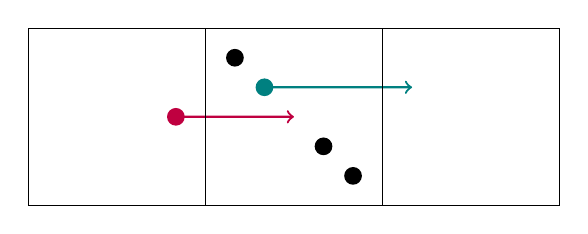
\begin{tikzpicture}[scale=0.75]
    \coordinate (a1) at (5.5,0.5);
    \coordinate (a2) at (5,1);
    \coordinate (a3) at (2.5,1.5);
    \coordinate (a4) at (4,2);
    \coordinate (a5) at (3.5,2.5);
    \draw[purple,->,thick] (a3) -- (4.5,1.5);
    \draw[teal,->,thick] (a4) -- (6.5,2);
    \draw (0,0) rectangle (3,3);
    \draw (3,0) rectangle (6,3);
    \draw (6,0) rectangle (9,3);
    \fill (a1) circle (0.15);
    \fill (a2) circle (0.15);
    \fill[purple] (a3) circle (0.15);
    \fill[teal] (a4) circle (0.15);
    \fill (a5) circle (0.15);
\end{tikzpicture}
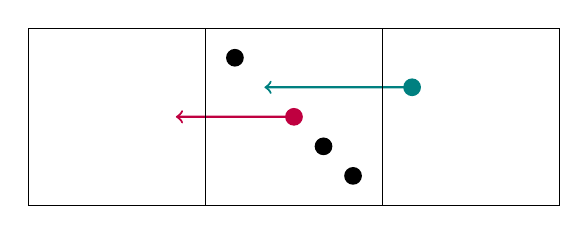
\begin{tikzpicture}[scale=0.75]
    \coordinate (a1) at (5.5,0.5);
    \coordinate (a2) at (5,1);
    \coordinate (a3) at (4.5,1.5);
    \coordinate (a4) at (6.5,2);
    \coordinate (a5) at (3.5,2.5);
    \draw[purple,->,thick] (a3) -- (2.5,1.5);
    \draw[teal,->,thick] (a4) -- (4,2);
    \draw (0,0) rectangle (3,3);
    \draw (3,0) rectangle (6,3);
    \draw (6,0) rectangle (9,3);
    \fill (a1) circle (0.15);
    \fill (a2) circle (0.15);
    \fill[purple] (a3) circle (0.15);
    \fill[teal] (a4) circle (0.15);
    \fill (a5) circle (0.15);
\end{tikzpicture}
\end{center}

Both maps move one point into and one out of $(1,0)$ at every step, so the number of elements in $(1,0)$ is fixed. Therefore the number of elements in the other column of the first two must be fixed. When mapping $\pi$ with $\Upsilon$ we take a certain amount of steps and when we map back with $\Upsilon^{-1}$ we take the same amount of steps, each cancelling out the steps of $\Upsilon$ and therefore $\Upsilon^{-1}(\Upsilon(\pi)) = \pi$ and similarly $\Upsilon\left(\Upsilon^{-1}(\pi')\right) = \pi'$ and thus, $\Upsilon$ is a bijection between $\textsf{Grid}_i(\mathcal{T}_1)$ and $\textsf{Grid}_i(\mathcal{T}_2)$.
\end{proof}

We can extend the Definition~\ref{def:slidable} of slidable tilings to any nonequal columns $c_1$ and $c_2$ instead of $0$ and $1$. The conditions would replace any constraints involving the first two columns with $c_1$ and $c_2$ and allow for subsequences on either side and between.

\begin{proposition}
Let $(\mathcal{T}_1,\mathcal{T}_2)$ be slidable in columns $c_1$ and $c_2$, then $|\textsf{Grid}_i(\mathcal{T}_1)| = |\textsf{Grid}_i(\mathcal{T}_2)|$ for all $i\in\N$.
\end{proposition}
\begin{proof}
Suppose the tilings have $c$ columns and let $\sigma = \sigma_1\sigma_2 \cdots \sigma_c \in \mathcal{S}_c$ where $\sigma_1 = c_1$ and $\sigma_2 = c_2$. We can permute the columns so $c_1$ and $c_2$ are the first two, slide them and permute back, that is we can use a composition of bijections, $C_{\sigma^{-1}} \circ \Upsilon \circ C_\sigma$, to map between the two.
\end{proof}